


\documentclass[english,11pt]{beamer}

\DeclareMathOperator{\Cov}{Cov}
\DeclareMathOperator{\Var}{Var}
\DeclareMathOperator{\E}{\mathbb{E}}
\DeclareMathOperator{\Proba}{\mathbb{P}}

\newcommand{\Covb}[2]{\ensuremath{\Cov\!\left[#1,#2\right]}}
\newcommand{\Eb}[1]{\ensuremath{\E\!\left[#1\right]}}
\newcommand{\Pb}[1]{\ensuremath{\Proba\!\left[#1\right]}}
\newcommand{\Varb}[1]{\ensuremath{\Var\!\left[#1\right]}}

% norm
\newcommand{\norm}[1]{\| #1 \|}

\newcommand{\indep}{\rotatebox[origin=c]{90}{$\models$}}





\usepackage{mathptmx,amsmath,amssymb,graphicx,bibentry,bbm,babel,ragged2e}

\makeatletter

\newcommand{\noun}[1]{\textsc{#1}}
\newcommand{\jitem}[1]{\item \begin{justify} #1 \end{justify} \vfill{}}
\newcommand{\sframe}[2]{\frame{\frametitle{#1} #2}}

\newenvironment{centercolumns}{\begin{columns}[c]}{\end{columns}}
%\newenvironment{jitem}{\begin{justify}\begin{itemize}}{\end{itemize}\end{justify}}

\usetheme{Warsaw}
\setbeamertemplate{footline}[text line]{}
\setbeamertemplate{headline}{}
\setbeamercolor{structure}{fg=purple!50!blue, bg=purple!50!blue}

\setbeamersize{text margin left=15pt,text margin right=15pt}

\setbeamercovered{transparent}


\@ifundefined{showcaptionsetup}{}{%
 \PassOptionsToPackage{caption=false}{subfig}}
\usepackage{subfig}

\usepackage[utf8]{inputenc}
\usepackage[T1]{fontenc}

\usepackage{multirow}

\usepackage{mdframed}


\AtBeginSection[]
{
  \begin{frame}
  \frametitle{Modèles de transport et modèles urbains}
  \tableofcontents[currentsection]
  \end{frame}
}

\makeatother

\begin{document}



\title{Integrating urban models and theories}

\author{J.~Raimbault$^{1,2,3,4}$\\
\texttt{juste.raimbault@ign.fr}
}


\institute{$^{1}$LASTIG, Univ Gustave Eiffel, IGN-ENSG\\
$^{2}$CASA, UCL\\
$^{3}$UPS CNRS 3611 ISC-PIF\\
$^{4}$UMR CNRS 8504 G{\'e}ographie-cit{\'e}s
}


\date{CSH Workshop - Cities as Complex Systems\\
20/06/2022
}


%Urban systems are highly multi-dimensional and complex, and thus studied from various perspectives and disciplines. To reach sustainable urban and territorial policies, we suggest that an integrative approach is needed. We propose in that context a theoretical and methodological framework, focused on the coupling and integration of simulation models.
%A first application example is then given, developing an urban dynamics model at the macroscopic scale coupling cities population dynamics with innovation diffusion. This simulation model allows investigating trade-offs between sustainable development goals in synthetic systems of cities, in particular emissions and innovation. Work in progress includes further model layers for economic exchanges and infrastructure, increasing the dimension of the SDG space in which Pareto compromises are found.
%The second example corresponds to the chapter of the Compendium discussed during this workshop. We review multiple models aiming at explaining regularities of city growth, including Gibrat‘s law of proportional random growth, Simon‘s random growth model, and more recent contributions. These models can be benchmarked against empirical evidence for multiple systems of cities, suggesting that a multi-modeling approach is more appropriate to cover the diversity of historical and geographical contexts observed for systems of cities.


\frame{\maketitle}


\section{Integration of urban models}




\sframe{Modeling urban complexity}{


\textit{Large scale urban models are intrinsically flawed and do not reach their goals of long-term application to planning}: \textbf{Requiem for large scale models in 1973} \cite{lee1973requiem}

\bigskip


\textit{Urban analytics and Smart Cities approaches may follow the same path if they ignore the past and the complexity of cities} \cite{batty2014can}


\bigskip


To foster relevance of large urban models:

\begin{itemize}
	\item Transparency on data and implementation, reproducibility
	\item Validation of models and sub-models: from small simple models well validated to larger integrated models
\end{itemize}

\medskip

$\rightarrow$ Open, reproducible urban models can be shared, coupled into modular integrated models, tested and validated \cite{banos2013pour}

}


\sframe{Proposed research framework}{

\justify

\textbf{Sustainable urban systems: } (i) multiple contradictory objectives; (ii) implemented by stakeholders at different scales, within various information and power contexts; (iii) adaptive on multiple time scales.


\bigskip

\textbf{Models are essential tools to } (i) capture complexity; (ii) construct integrated perspectives; (iii) link data, empirical stylised facts and decision-making.

\bigskip


$\rightarrow$ \textbf{Integrated models} to simulate multiple dimensions of \textbf{urban systems} towards decision-making in the context of \textbf{sustainable transitions}.

\bigskip

\begin{itemize}
	\item Horizontal integration (model coupling and interdisciplinarity)
	\item Vertical integration (multi-scale models)
	\item Model exploration and validation methods
\end{itemize}


}



\sframe{Horizontal integration: interdisciplinarity}{

\textit{Literature mapping and systematic review tools to enhance integration}

\medskip

\begin{center}
	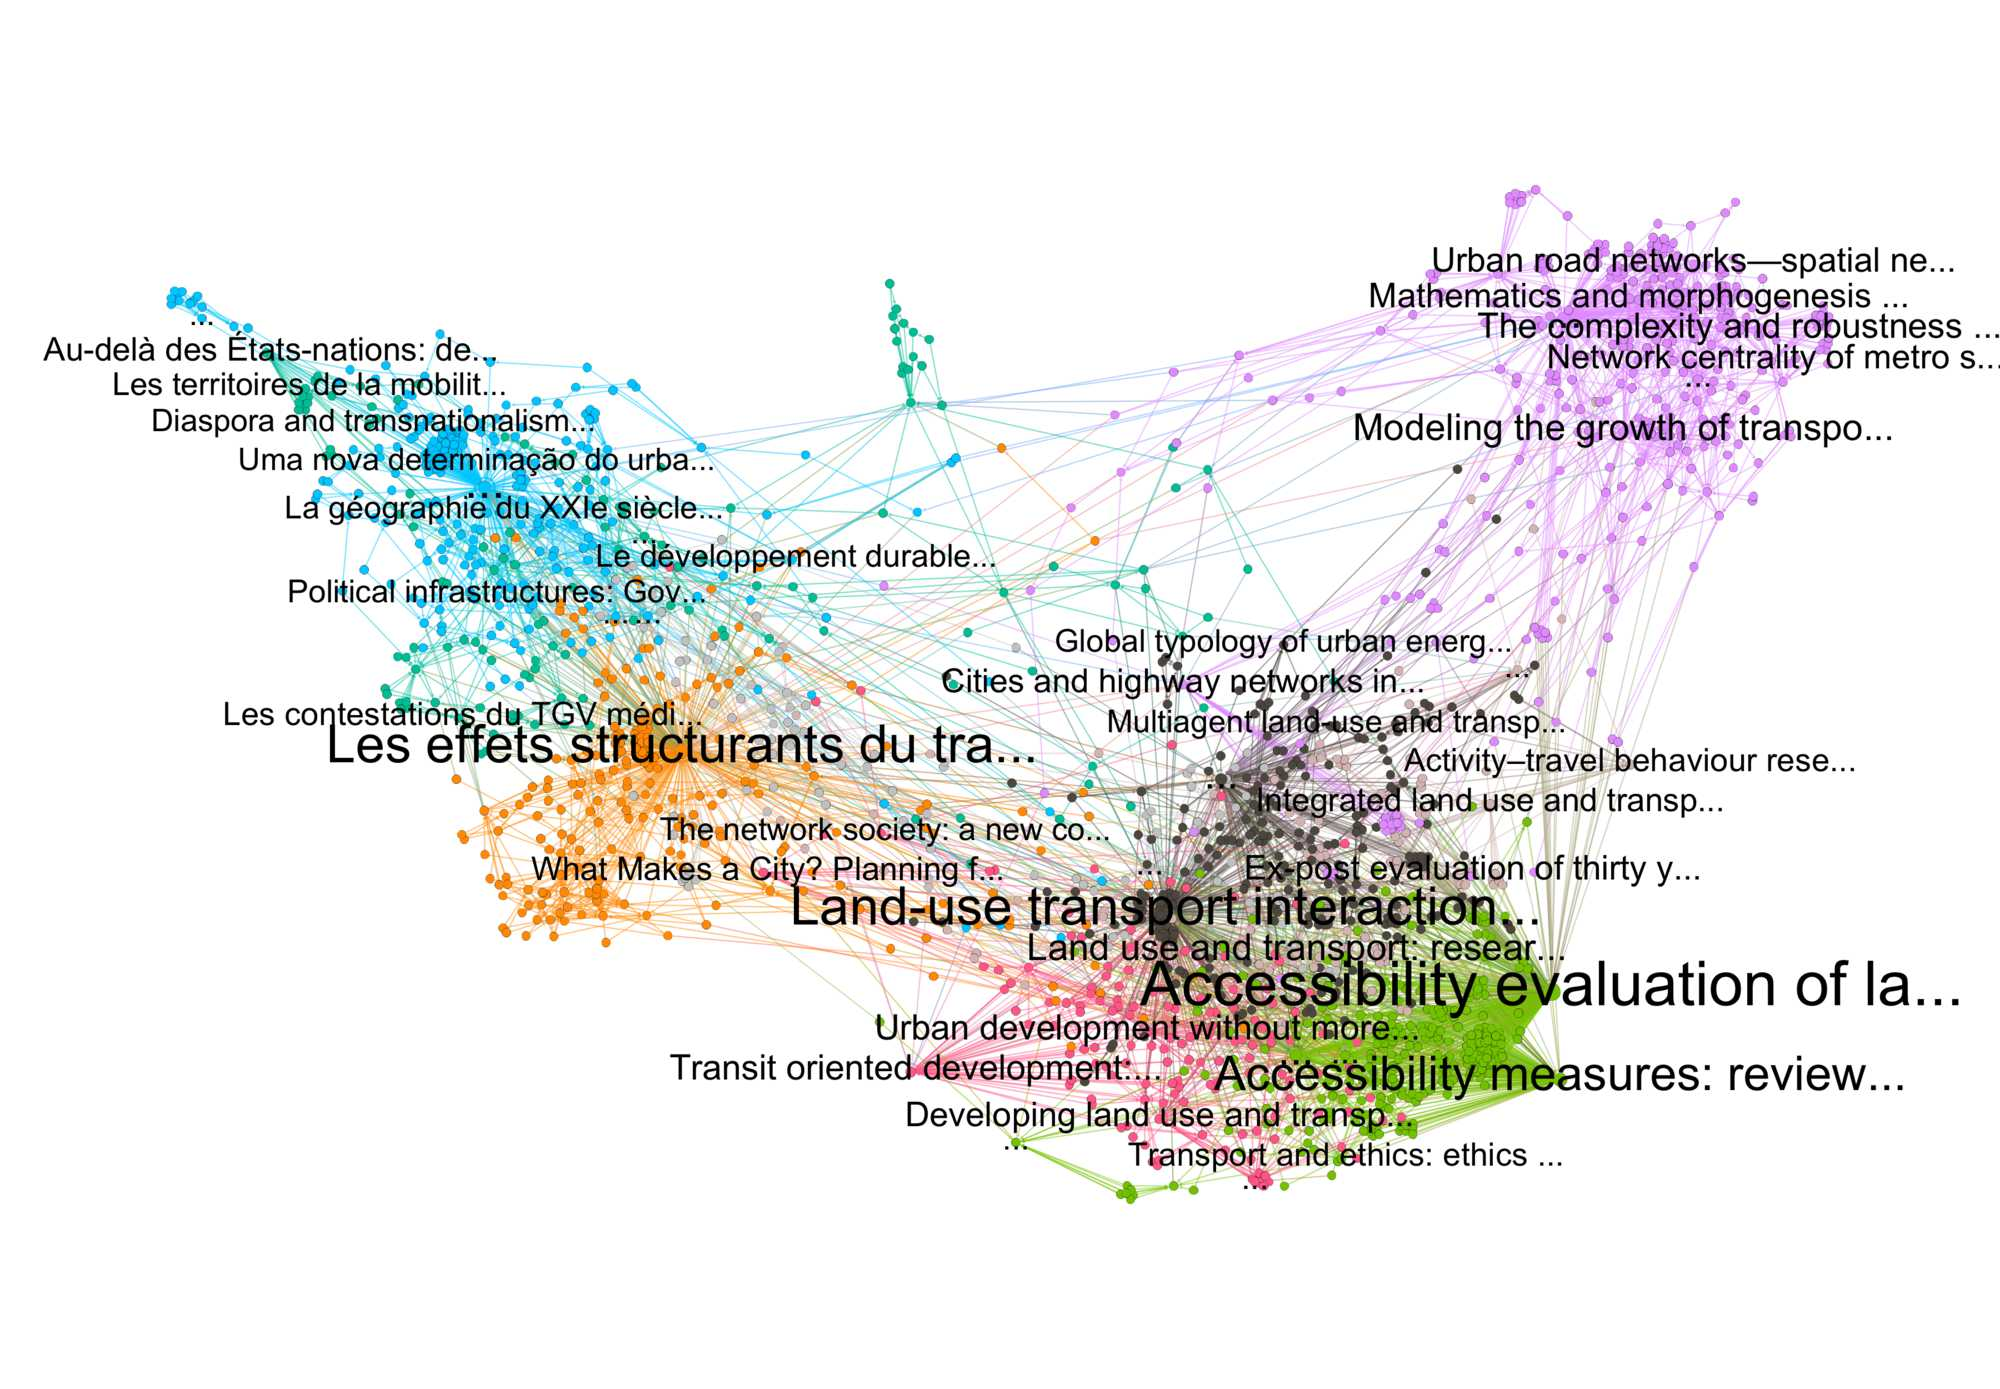
\includegraphics[width=0.9\textwidth,trim={0 2cm 0 2cm},clip]{figures/2-2-2-fig-quantepistemo-citnw.jpg}	
\end{center}

\medskip

\tiny

\vspace{-1cm}

Raimbault, J. (2019). Exploration of an interdisciplinary scientific landscape. Scientometrics, 119(2), 617-641.

\nocite{raimbault2019exploration}

}



\sframe{Implementing horizontal model integration}{

\justify

\textbf{Work in progress:} \textit{constructing a multimodal four step transport models by linking open components and data with scientific workflow engines}

\bigskip

\textbf{Integrated models:}

\begin{itemize}
	\item MATSim model (MATSim Community) for transport \cite{w2016multi}
	\item SPENSER model (University of Leeds) for synthetic population \cite{spooner2021dynamic}
	\item QUANT model (CASA, University College London) for spatial interactions \cite{batty2021new}
	\item spatialdata library (OpenMOLE community) for data processing \cite{raimbault2020scala}
\end{itemize}

\smallskip

\tiny

Raimbault, J., \& Batty, M. (2021). Estimating public transport congestion in UK urban areas with open transport models. GISRUK 2021 Proceedings.

\nocite{raimbault2021estimating}

}


\sframe{Horizontal integration: multi-modeling and benchmarks}{


\begin{center}
	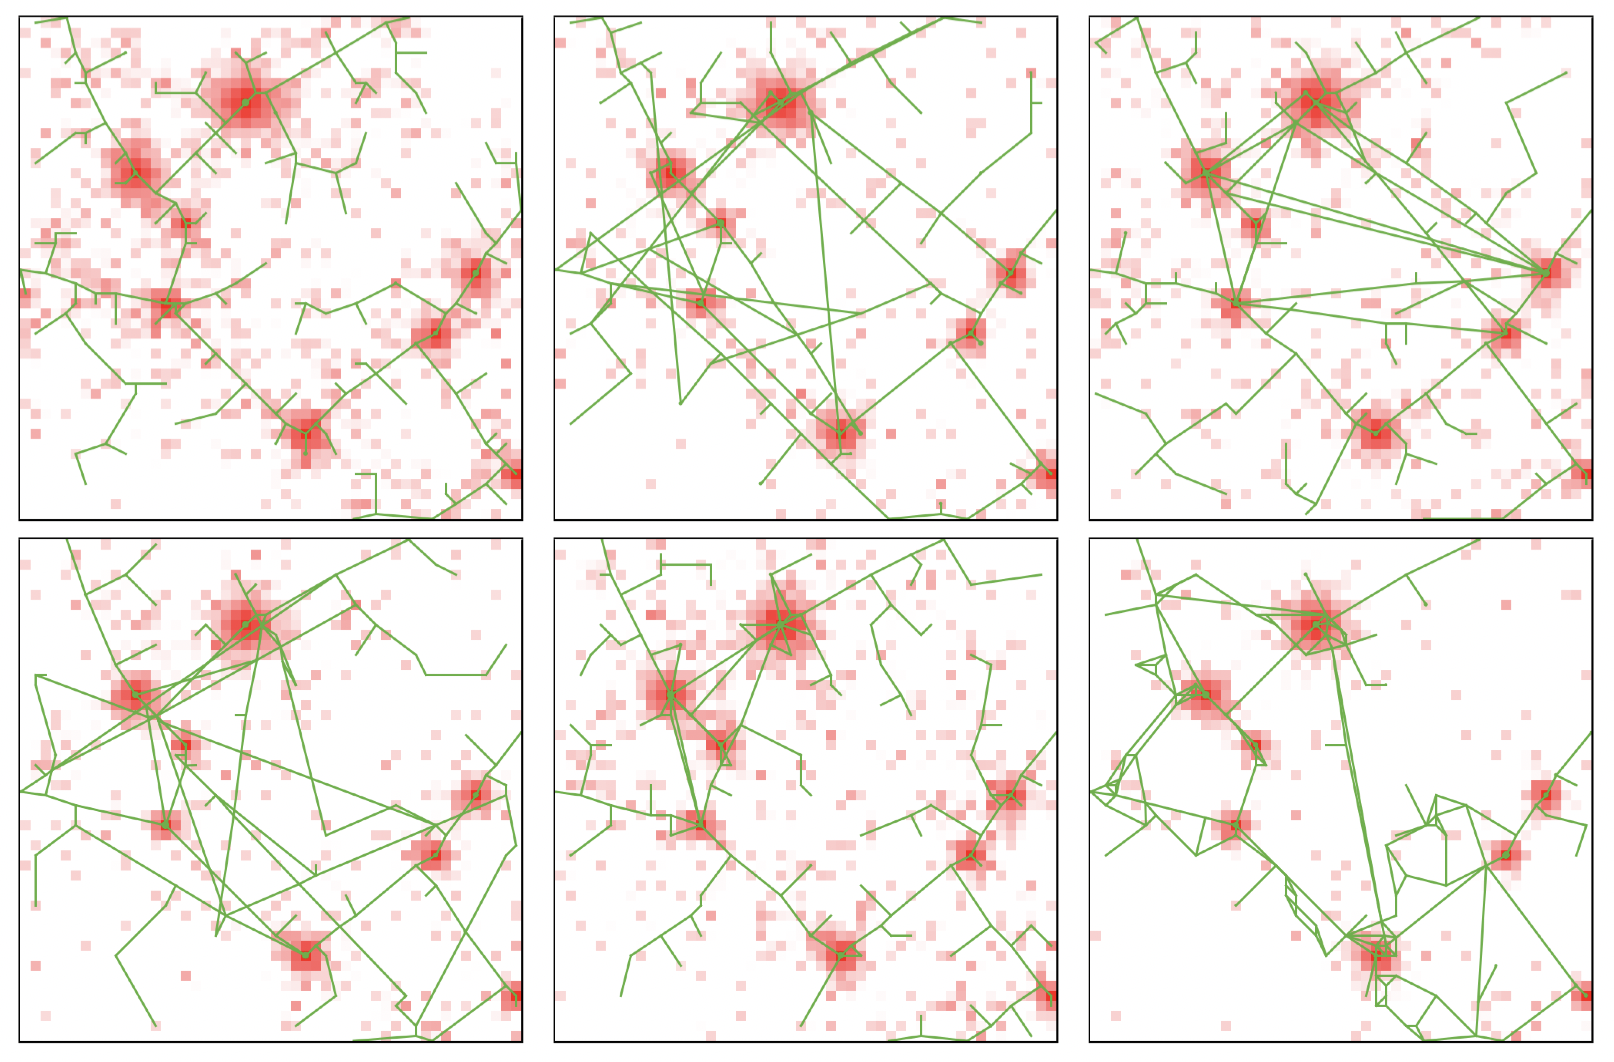
\includegraphics[width=0.56\linewidth]{figures/meso_multimodeling.png}\hspace{0.5cm}
	
\includegraphics[width=0.36\linewidth]{figures/mesobench_Fig3.png}
\end{center}

\medskip

\textit{Benchmarking network and urban morphogenesis models}


\medskip

\tiny

Raimbault, J. (2018). Multi-modeling the morphogenesis of transportation networks. In Artificial Life Conference Proceedings (pp. 382-383). MIT Press, Cambridge.

\nocite{raimbault2018multi}

\smallskip

Raimbault, J. (2020). A comparison of simple models for urban morphogenesis. arXiv preprint arXiv:2008.13277.

\nocite{raimbault2020comparison}

\smallskip

Raimbault, J. (2021). Complementarity of generative models for road networks. arXiv preprint arXiv:2109.15206.

\nocite{raimbault2021complementarity}



}




\sframe{Vertical integration: towards multi-scale models}{



\begin{center}
	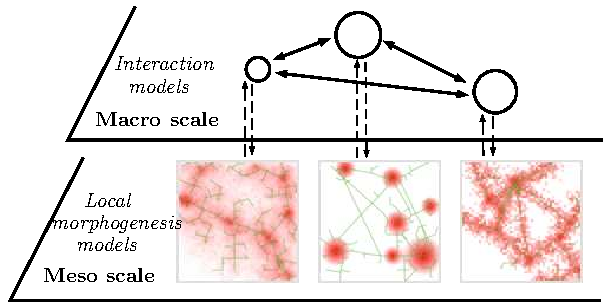
\includegraphics[width=0.75\textwidth]{figures/multiscale_morph.pdf}
\end{center}

\medskip

\textit{Processes specific to scales, coupling implies dedicated ontologies} 

\medskip

\tiny

Raimbault, J. (2021). Strong coupling between scales in a multi-scalar model of urban dynamics. arXiv preprint arXiv:2101.12725.

\nocite{raimbault2021strong}

\smallskip

Raimbault, J. (2021). A multiscale model of urban morphogenesis. arXiv preprint arXiv:2103.17241.

\nocite{raimbault2021multiscale}


}




\sframe{Model exploration methods to foster knowledge integration}{
	
	OpenMOLE software \cite{reuillon2013openmole}: \textit{(i) Innovative exploration methods; (ii) Scaling of methods on high performance computing environments; (iii) Scripts to embed and couple models.}
	
	\smallskip
	
	\centering
	
	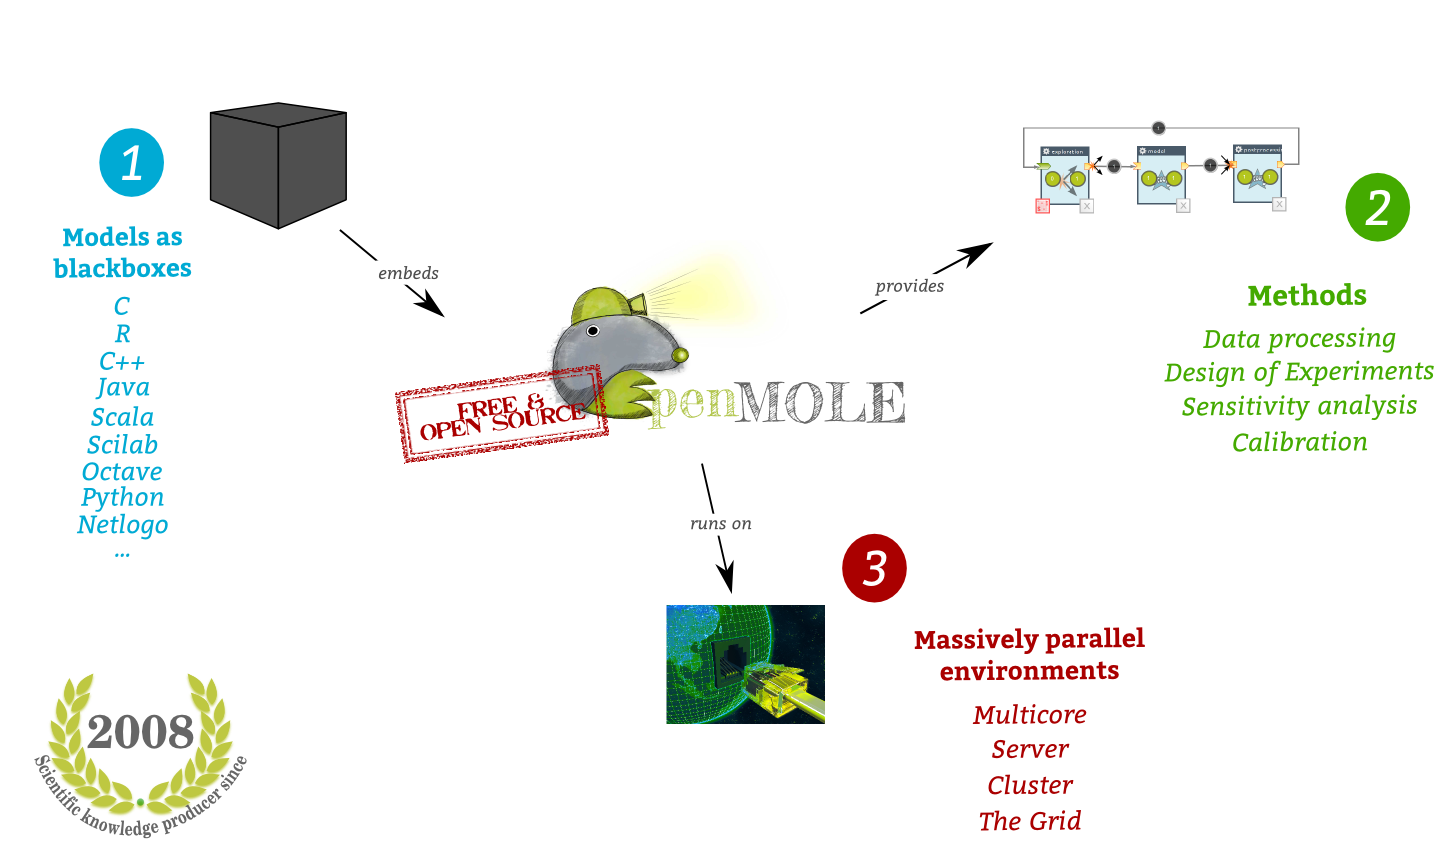
\includegraphics[width=0.8\textwidth]{figures/openmoleGal.png}
	
}




\sframe{Validation: towards spatial sensitivity analysis}{



\centering

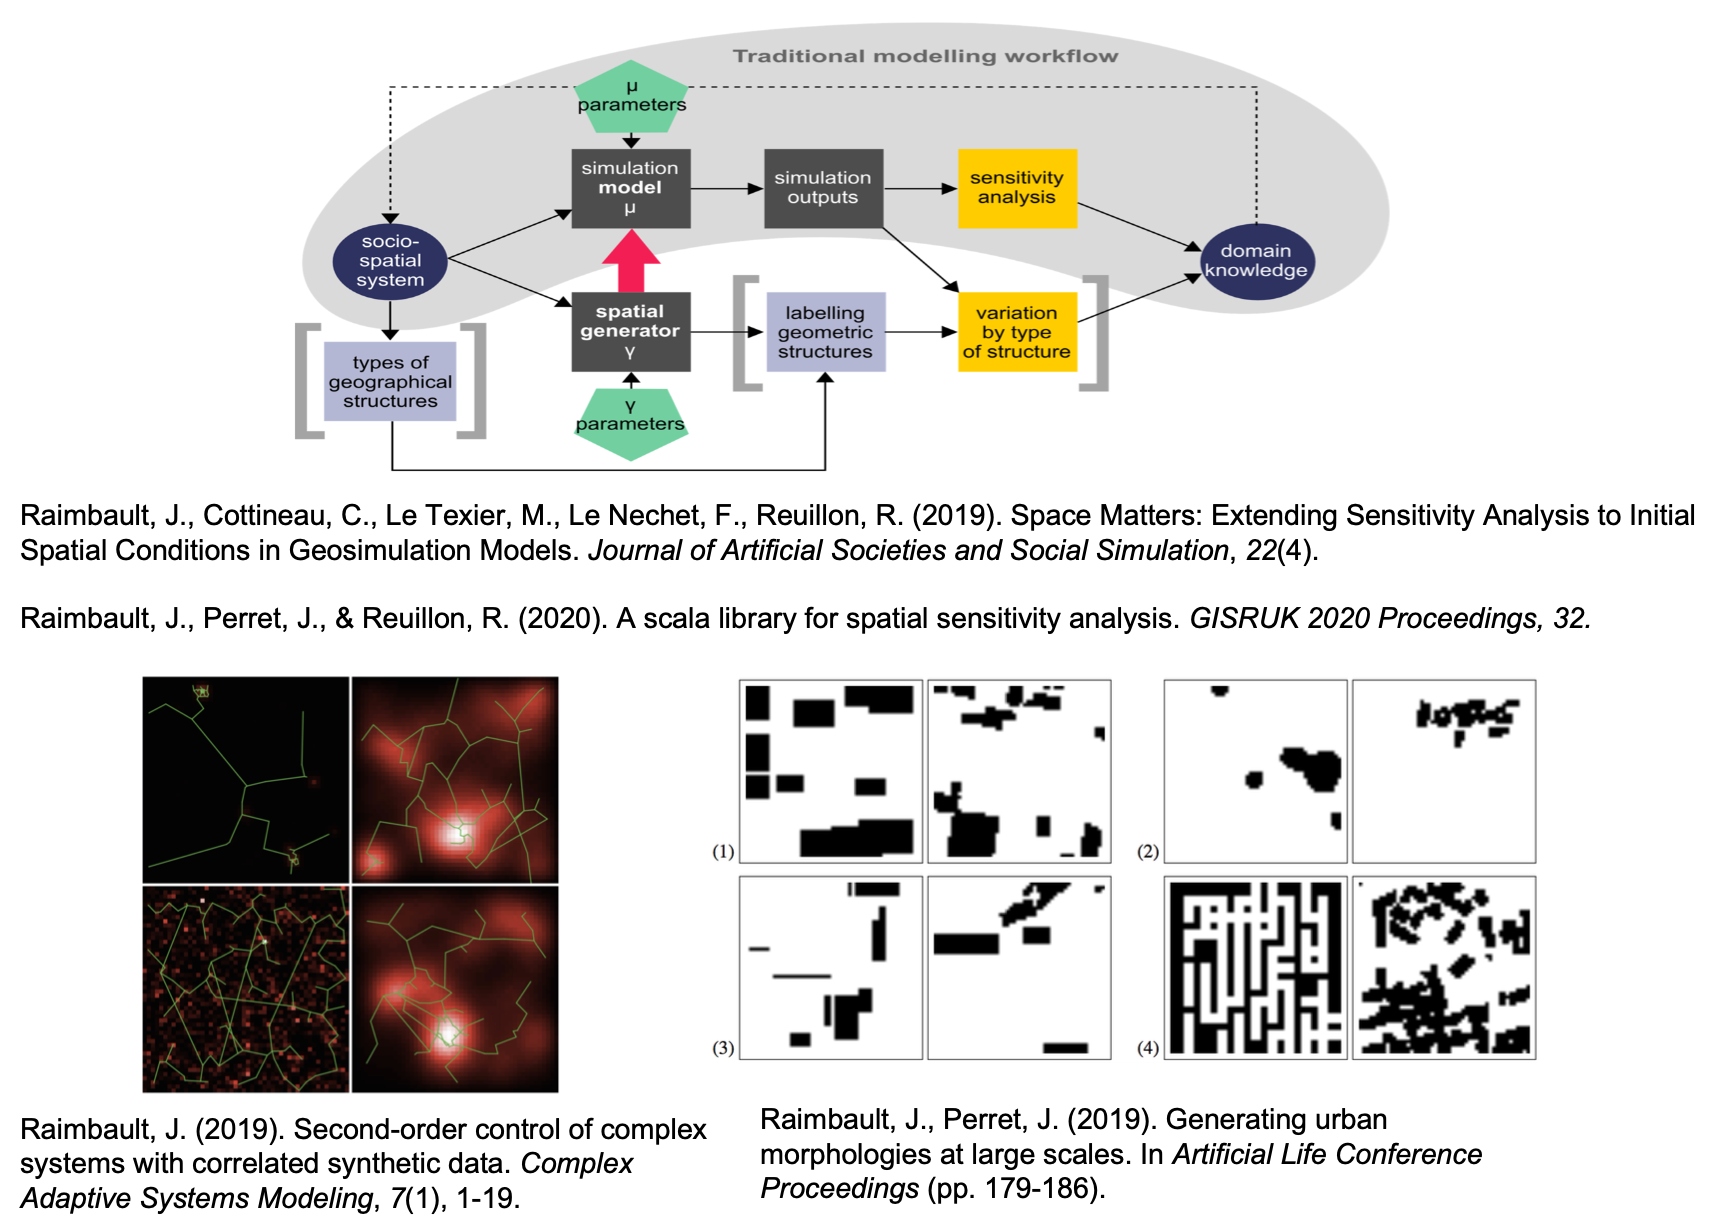
\includegraphics[width=0.95\linewidth]{figures/spatial_sa.png}

\nocite{raimbault2019second}
\nocite{raimbault2019generating}
\nocite{raimbault2019space}

}






\section{Urban dynamics: trade-offs between SDGs}




\sframe{Cities and SDGs}{

\justify

\textbf{SDG 11}: ``Make cities and human settlements inclusive, safe, resilient, and sustainable'' \cite{nations2015sustainable}

\bigskip

$\rightarrow$ Environmental Kuznet Curve hypothesis \cite{dinda2004environmental, stern2004rise}: inverted U-shaped relationship between environmental impact and income per-capita; not validated empirically \cite{harbaugh2002reexamining}

\bigskip

$\rightarrow$ Trade-offs between SDGs in urban systems \cite{viguie2012trade}


}



\sframe{Innovation diffusion and urban dynamics}{

$\rightarrow$ \textbf{Innovation diffusion} is a crucial process in artificial life evolutionary systems and open-ended evolution \cite{bedau2000open}

\medskip

$\rightarrow$ Artificial societies used to study the dynamics of innovation \cite{zenobia2009artificial}

\medskip

$\rightarrow$ Innovations diffuse hierarchically in systems of cities \cite{hagerstrand1968innovation}, potential explanation of urban scaling laws \cite{pumain2006evolutionary}

\bigskip

\textit{Innovation diffusion as a privileged entry to understand urban evolution}


}



\sframe{Model rationale}{


\begin{itemize}
	\item Agents are cities, macroscopic scale (regional, country, continental) and long time scales (century)
	\item Cities characterised by their size in terms of population; genome as adoption proportions of innovations (social or technological) for each city (one single dimension to simplify)
	\item Following \cite{favaro2011gibrat}, attractivity of cities due to level of innovation drive their population growth through spatial interactions; innovation diffuse through an other spatial interaction model \cite{fotheringham1989spatial}
	\item Mutations occur in cities as new innovations appear
\end{itemize}

}




\sframe{Model description}{
\centering
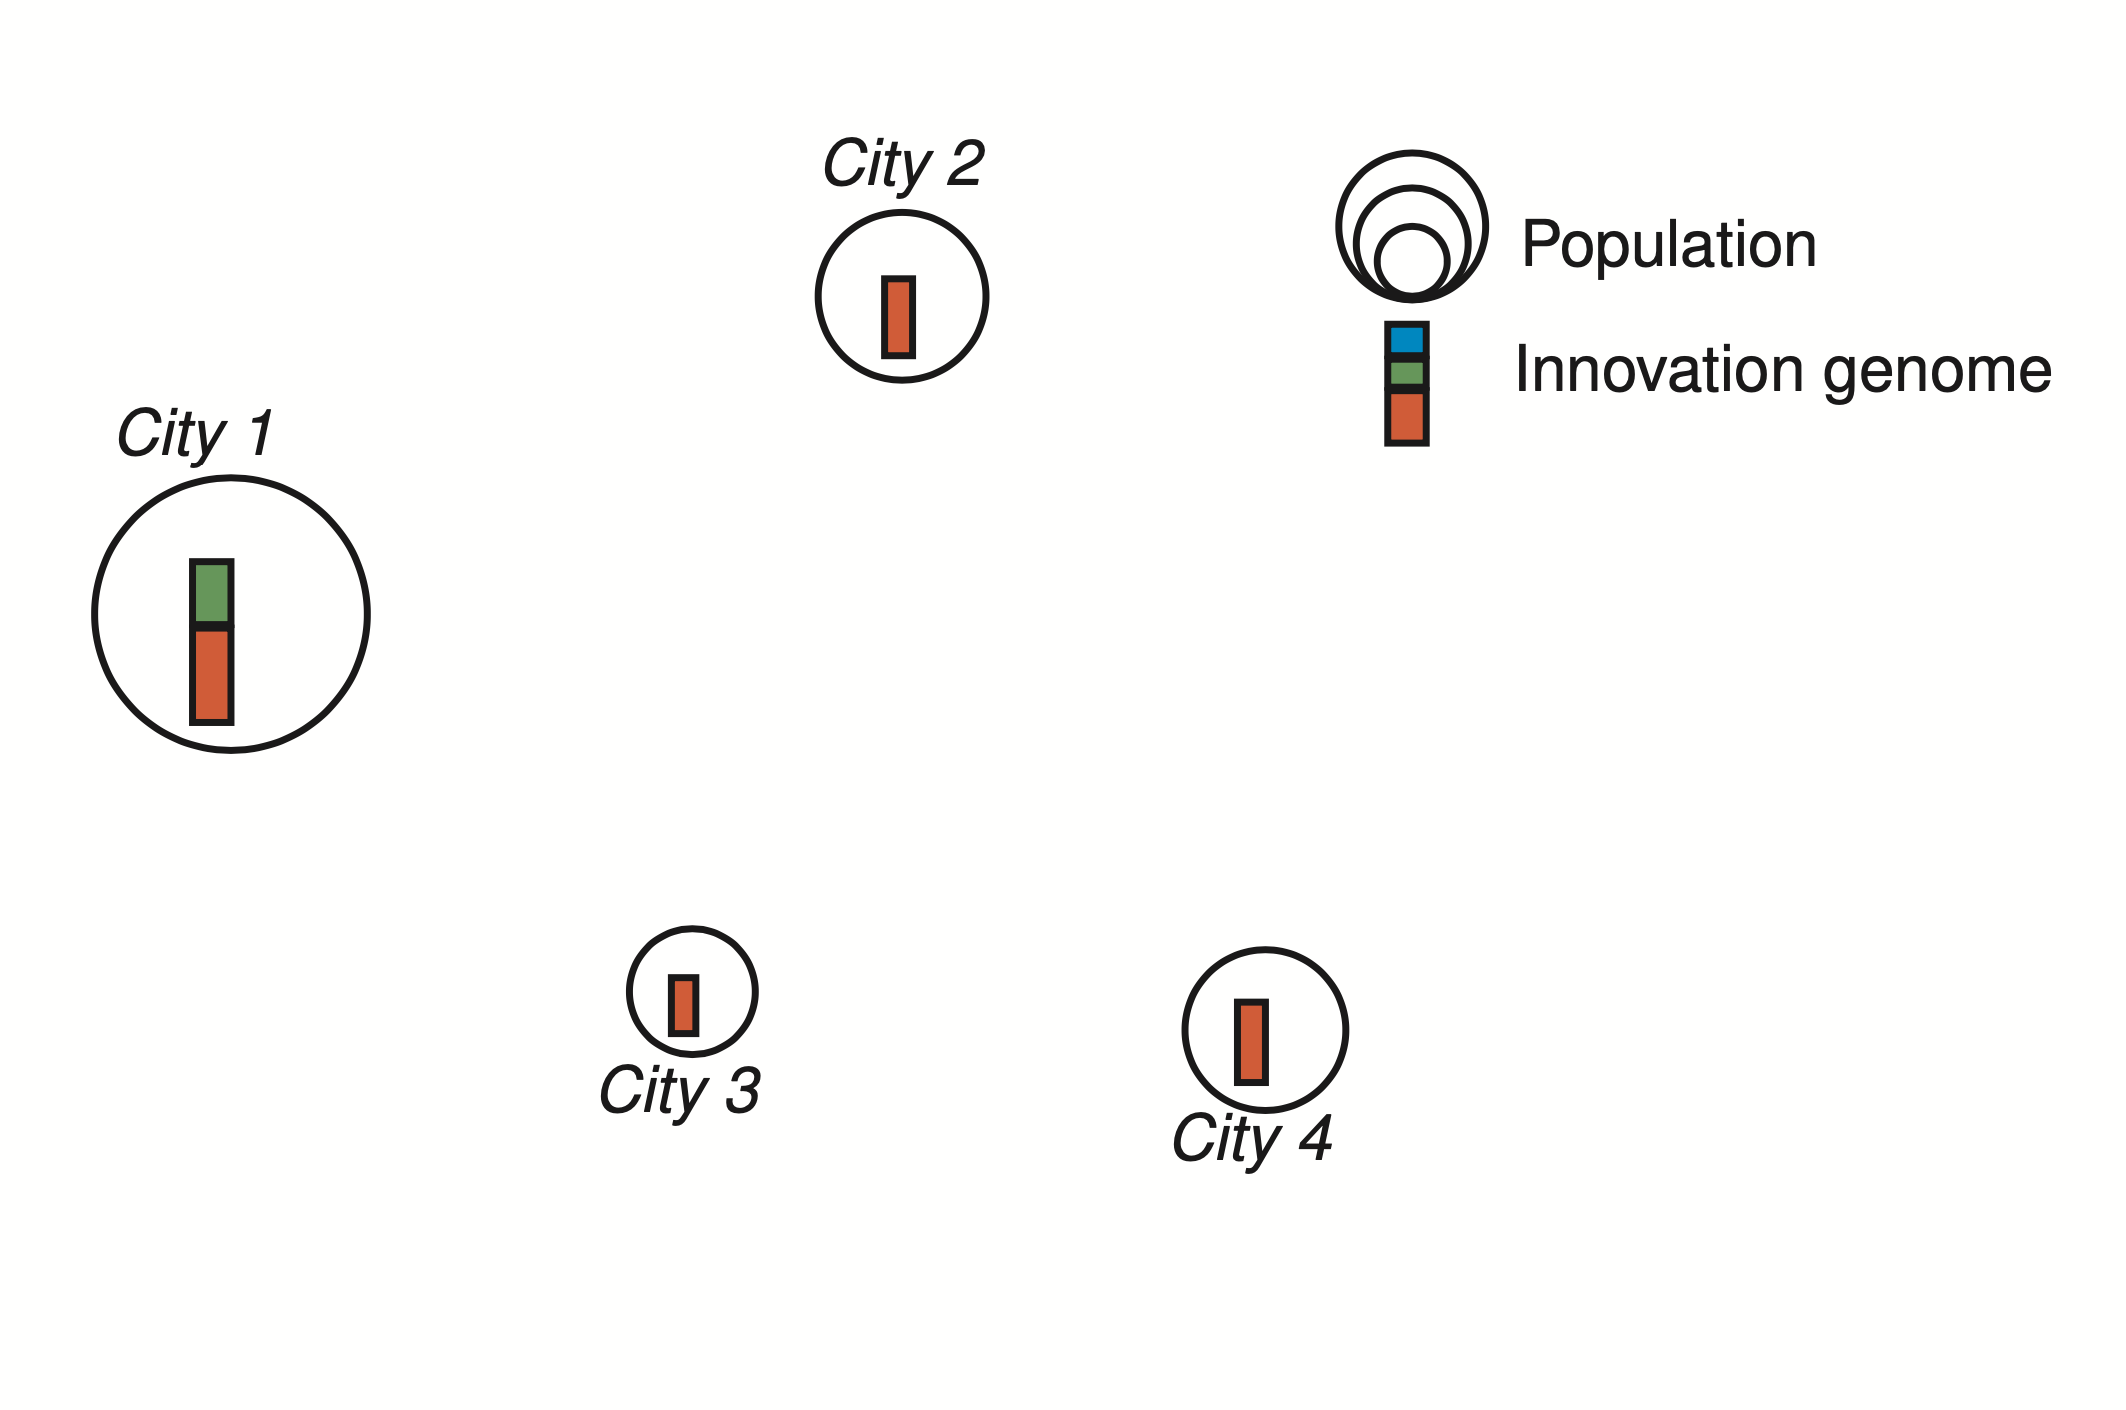
\includegraphics[width=\linewidth]{figures/model_1.png}
}

\sframe{Model description}{
\centering
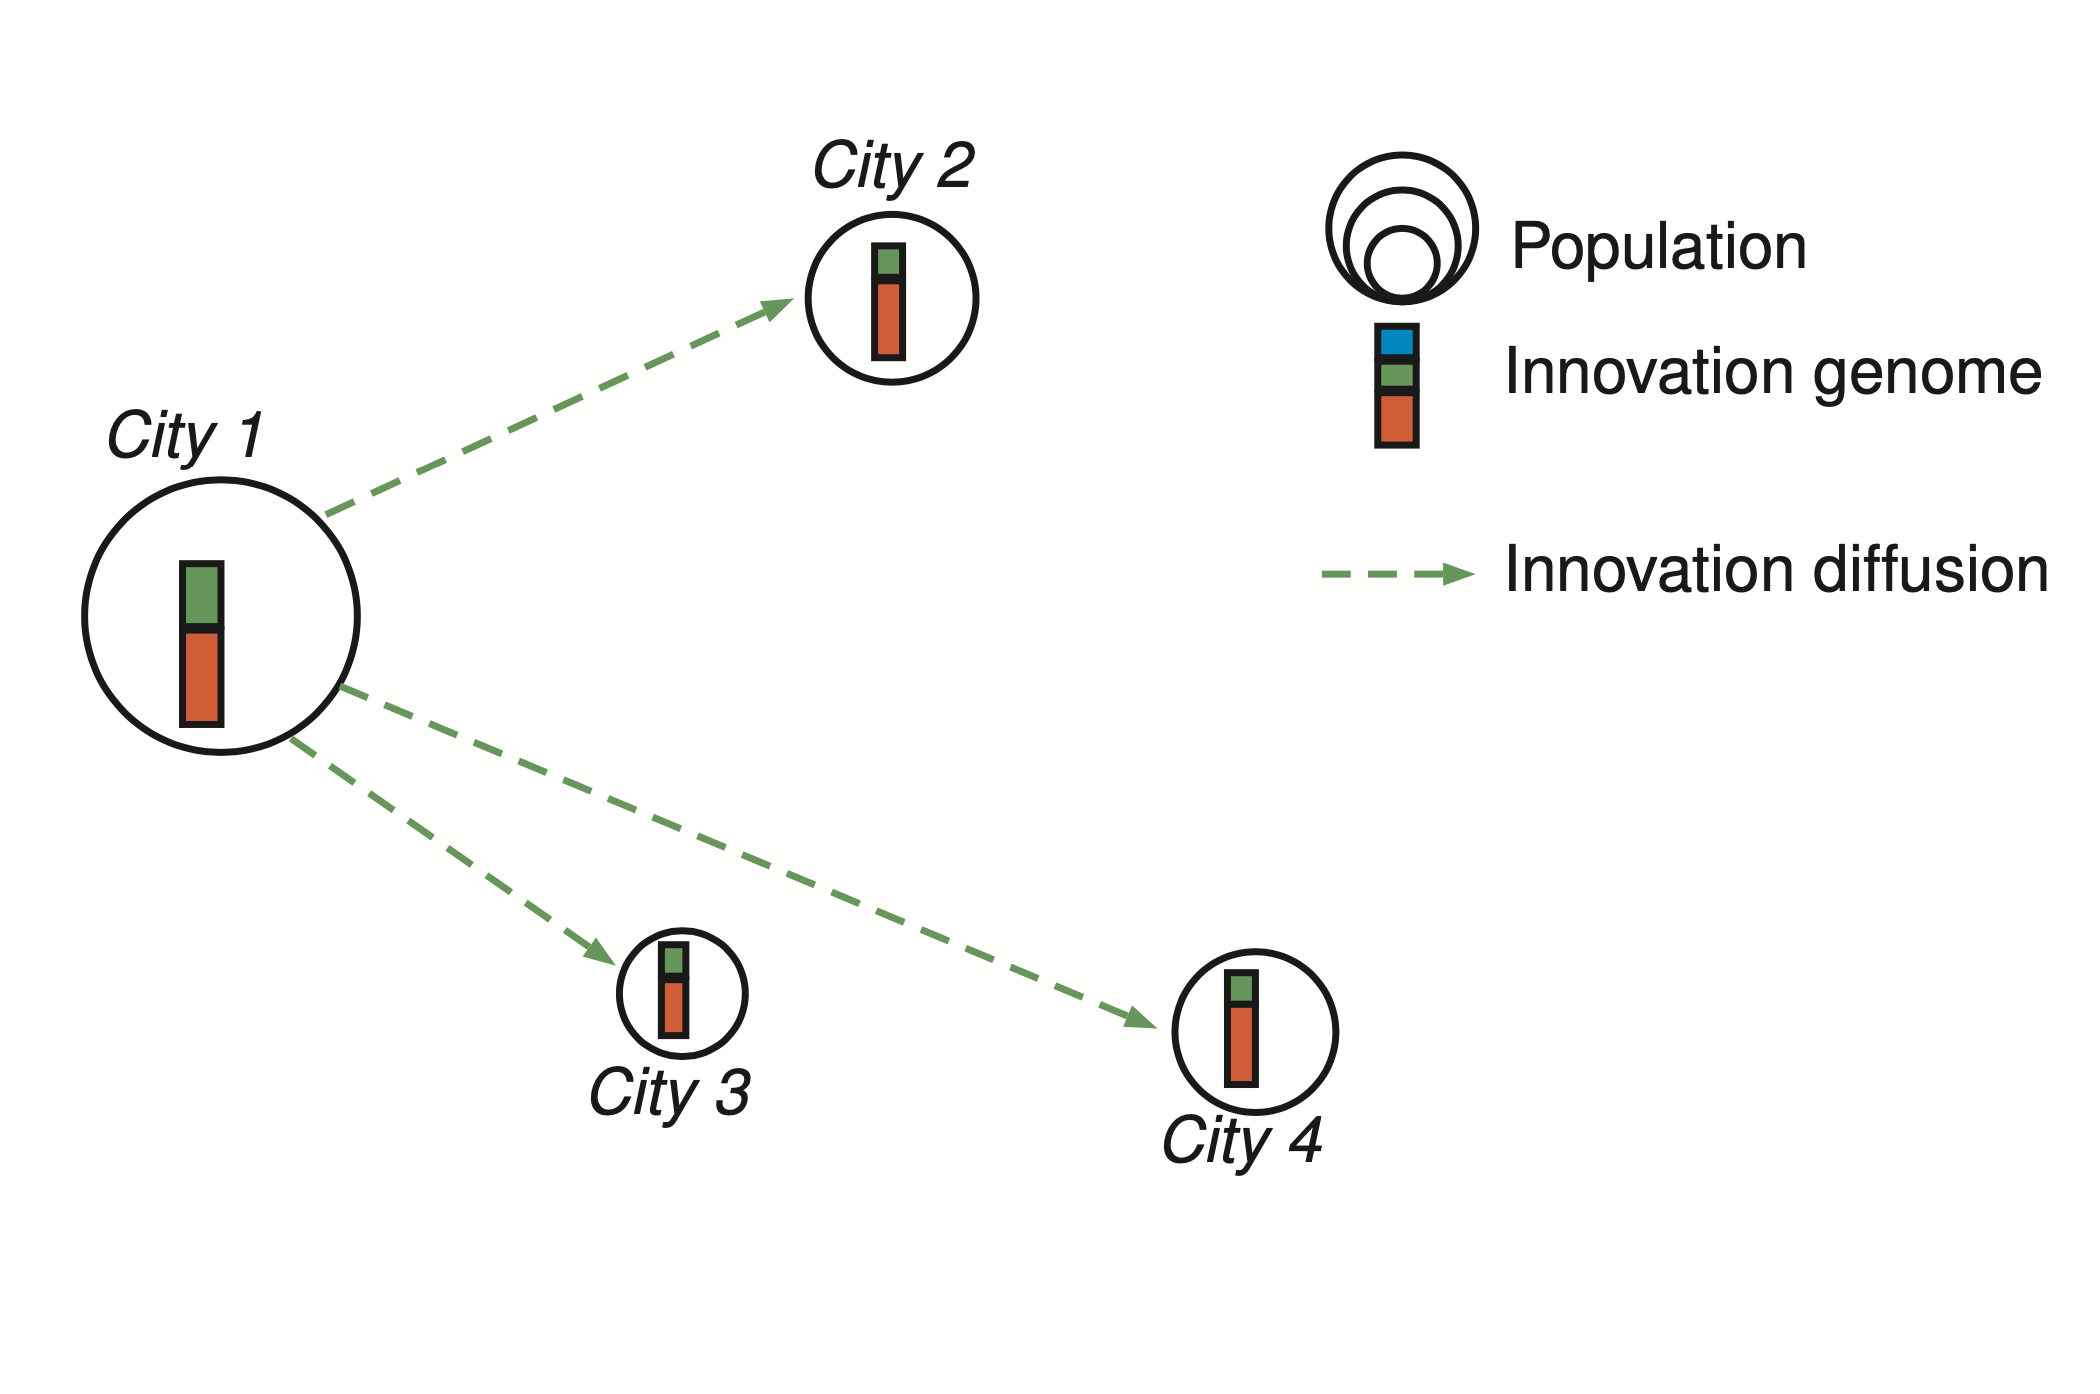
\includegraphics[width=\linewidth]{figures/model_2.png}
}

\sframe{Model description}{
\centering
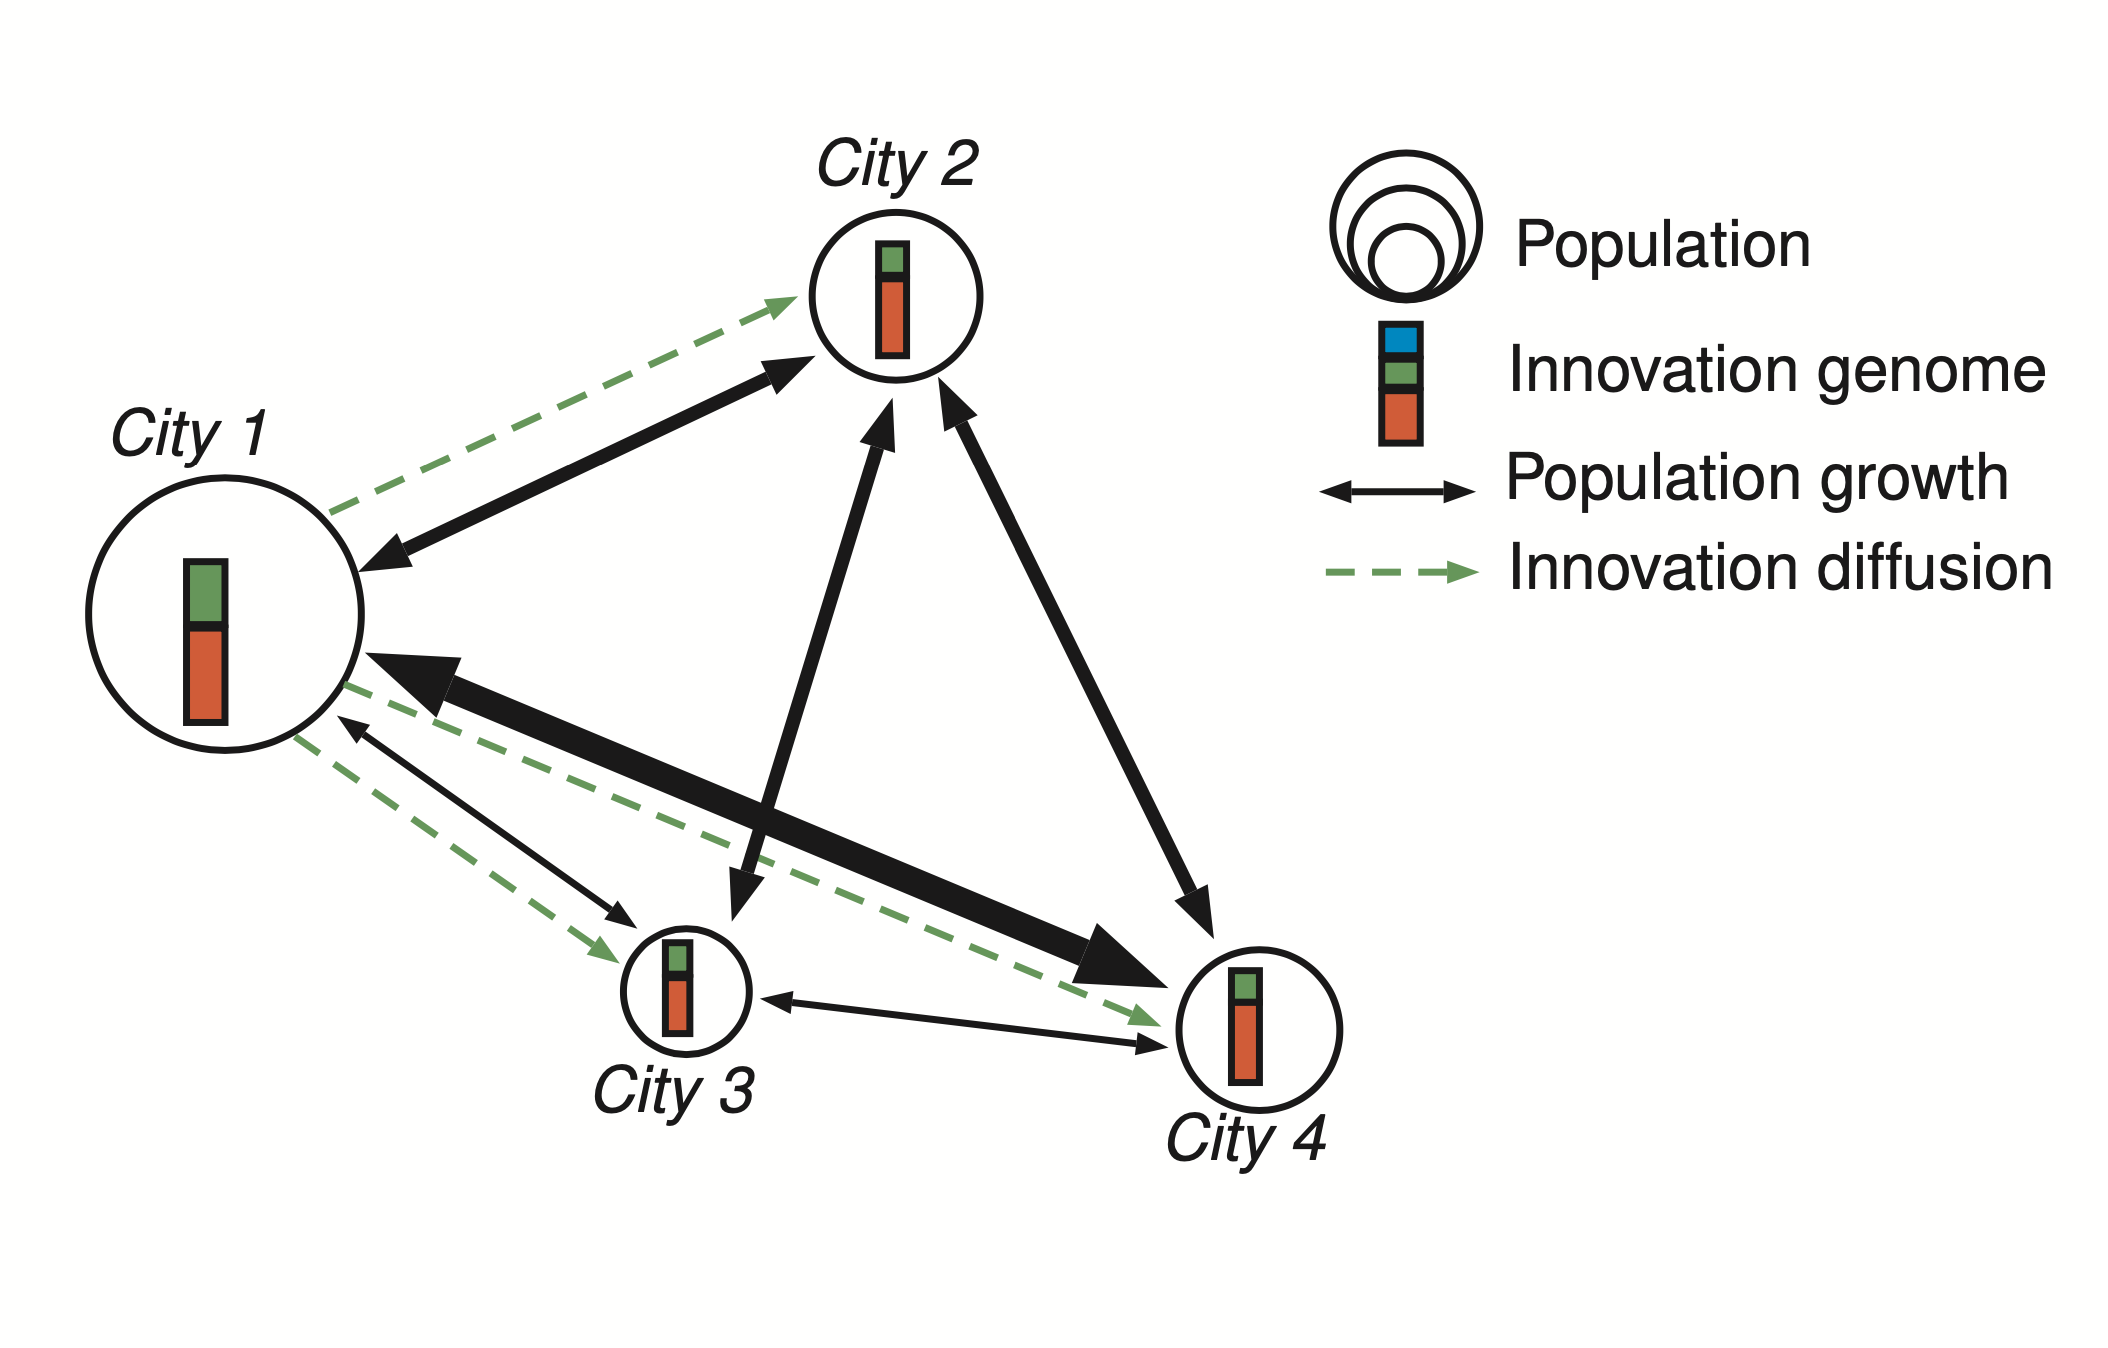
\includegraphics[width=\linewidth]{figures/model_3.png}
}

\sframe{Model description}{
\centering
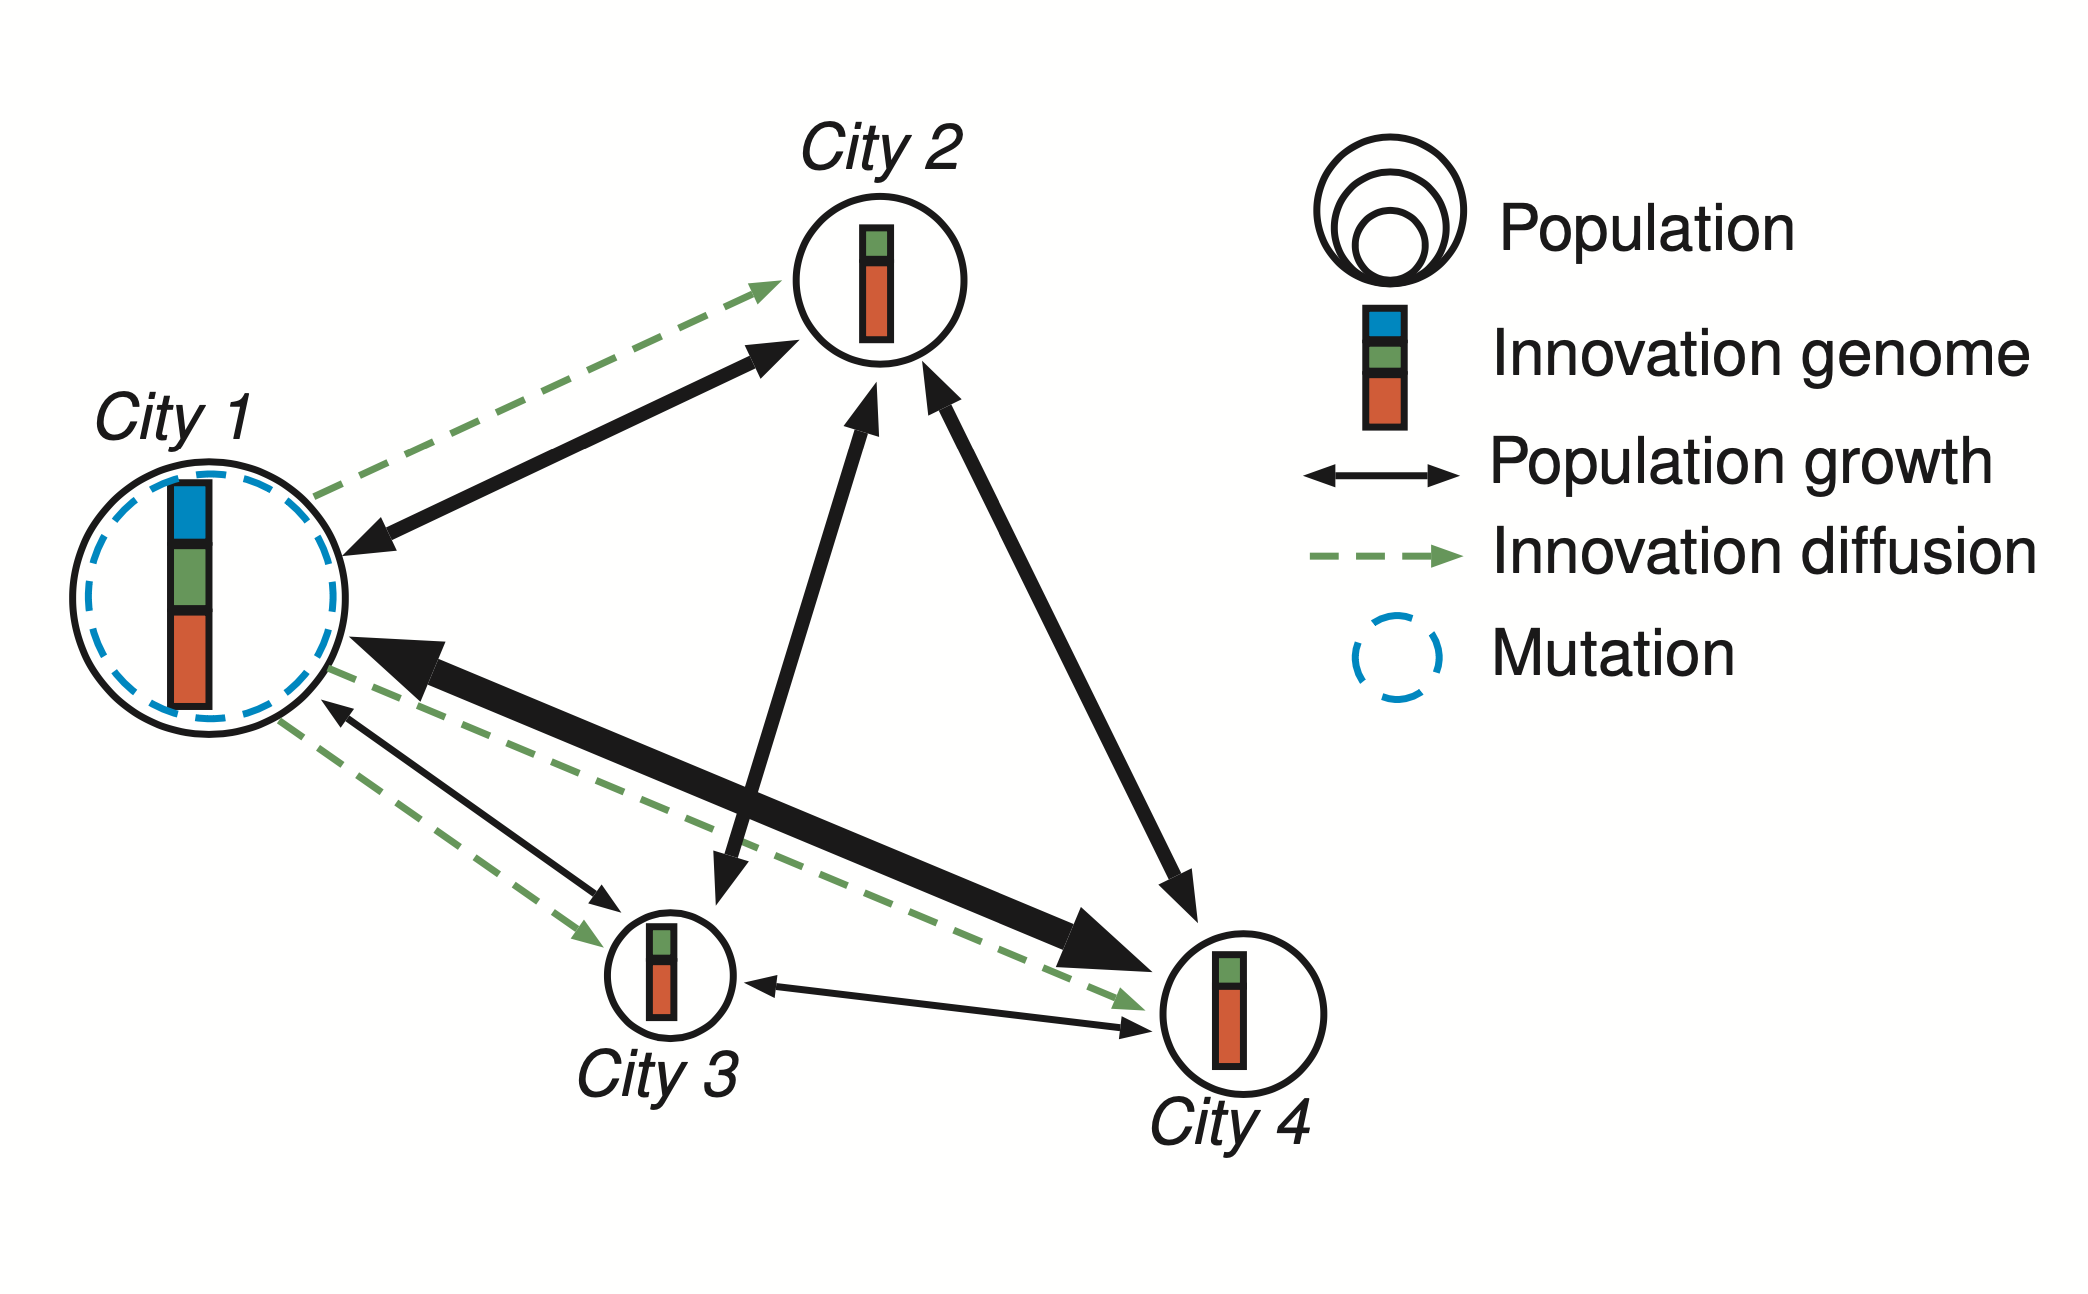
\includegraphics[width=\linewidth]{figures/model_4.png}
}



\sframe{Model formalisation}{


At each time step, with $P_i \left(t\right)$ population, $\delta_{c,i}\left(t\right)$ genome, $u_c$ utility of innovation, $p_{c,i,t}$ share of total population adopting innovation $c$ in city $i$
\begin{enumerate}
	\item Crossover through the diffusion of innovations
	\[
	\delta_{c,i,t} \textrm{ = } \frac{\sum_j p_{c,j,t-1}^{\frac{1}{u_c}} \cdot \exp{\left(-\frac{d_{ij}}{d_I}\right)}}{\sum_c \sum_j p_{c,j,t-1}^{\frac{1}{u_c}} \cdot \exp{\left(-\frac{d_{ij}}{d_I}\right)}}	
	\]
	\item Population growth through spatial interactions $P_i\left(t\right) - P_i\left(t-1\right) \textrm{ = } w_I\cdot \sum_j \frac{V_{ij}}{<V_{ij}>}$ with
	\[ 
	V_{ij} \textrm{ = } \frac{P_{i}\left(t-1\right) \cdot P_{j}\left(t-1\right)}{\left(\sum_k P_k\left(t-1\right)\right)^2} \cdot \exp{\left(-\frac{d_{ij}}{d_G} \cdot \prod_c \delta_{c,i,t}^{\phi_{c,t}}\right)}
	\]
	and $\phi_{c,t} \textrm{ = } \sum_i \delta_{i,c,t}\cdot P_i\left(t-1\right) /\sum_{i,c} \delta_{i,c,t}\cdot P_{i}\left(t-1\right)$
	\item Mutations with innovations introduced with probability $\beta \cdot \left(P_i \left(t\right) / \max_k P_k \left(t\right)\right)^{\alpha_I}$ and an initial penetration rate $r_0$; new utility $u_c$ randomly distributed (normal or log-normal) with average current average utility and standard deviation a given parameter $\sigma_U$
\end{enumerate}



}


%\sframe{Model indicators}{

%\begin{itemize}
%	\item Average diversity
%	\[
%	D \textrm{ = } \frac{1}{t_f \textrm{+} 1} \sum_{t\textrm{=}0}^{t_f} \left(1 - \sum_{i,c} \left(p_{c,i,t}\right)^2 \right)	
%	\]
%	\item Average utility
%	\[
%	U \textrm{ = } \frac{1}{t_f \textrm{ + } 1} \sum_{t \textrm{=}0}^{t_f} \sum_{i,c} \delta_{c,i,t} u_c 
%	\]
%	\item Innovatitivity 
%	\[
%	I \textrm{ = } \frac{\max c}{N\cdot \left(t_f \textrm{ + } 1\right)}
%	\]
%	\item Population trajectories, summarized by final hierarchy \cite{raimbault2020unveiling}
%\end{itemize}
%}



\sframe{Synthetic configurations}{

Model applied on synthetic systems of cities (so that conclusions are independent of geographical contingencies \cite{raimbault2019space}):

\medskip

\begin{itemize}
	\item random positions and rank-size hierarchy $P_i \left(0\right) \textrm{ = } \frac{P_{max}}{i^{\alpha_0}}$ with $\alpha_0 \textrm{ = } 1.0$ and $P_{max} \textrm{ = } 100,000$
	\item regional urban system scale: $N \textrm{ = } 30$ cities
	\item simulated for $t_f \textrm{ = } 50$ macroscopic time steps (order of magnitude of a century)
\end{itemize}



}


%
%\sframe{Model parameters}{
%
%\centering
%
%	\begin{tabular}{|l|l|l|l|l|l|}
%	\hline
%	Parameter & Not. & Process & Range & Def. \\ \hline
%	Number of cities & $N$ & Spatial scale & $[10 ; 100]$ & $30$\\
%	Initial hierarchy & $\alpha_0$ & System of cities & $[0.5 ; 2.0]$ & $1$\\
%	Initial population & $P_{max}$ & System of cities & $[10^4 ; 10^7]$ & $10^5$\\
%	Simulation steps & $t_f$ & Temporal scale & $[10 ; 100]$ & $50$\\
%	Growth rate & $w_I$ & Pop. growth & $[0.001 ; 0.01]$ & $0.005$\\\hline
%	Gravity range & $d_G$ & Crossover & $[0 ; 2]$ & $1$\\
%	Innovation range & $d_I$ & Crossover & $[0 ; 2]$ & $1$\\
%	Innovation rate & $\beta$ & Mutation & $[0 ; 1]$ & $0.5$\\
%	Innovation hierarchy & $\alpha_I$ & Mutation & $[0 ; 2]$ & $1$\\
%	Innov. utility std. & $\sigma_U$ & Mutation & $\left[ 0.7;2\right]$ & $1$\\
%	Penetration rate & $r_0$ & Mutation & $\left[0.1;0.9\right]$ & $0.5$\\
%	Utility type & - & Mutation & \{n;ln\}& ln \\
%	\hline
%	\end{tabular}
%
%
%}


%
%\sframe{Implementation}{
%
%\justify
%
%Model implemented in \texttt{scala}; relatively large parameter space
%
%\medskip
%
%$\rightarrow$ integration into the OpenMOLE model exploration open source software \cite{reuillon2013openmole}
%
%\begin{center}
%
\includegraphics[height=0.13\textheight]{figures/iconOM.png}
%
\includegraphics[height=0.13\textheight]{figures/openmole.png}
%\end{center}
%
%
%\textit{Enables seamlessly (i) model embedding; (ii) access to HPC resources; (iii) exploration and optimization algorithms}
%
%\medskip
%
%\url{https://openmole.org/}
%
%
%}




\sframe{Trade-offs between SDGs}{

\justify

$\rightarrow$ \textit{Which trade-offs between innovation (SDG 9: innovation) and emissions (SDG 14: climate) in systems of cities?}

\bigskip

Application of the urban evolution model, optimising with NSGA2 for conflicting objectives in synthetic systems of cities:

\medskip

\begin{enumerate}
   \item total utility of innovations 
 \[
 U = \sum_{t,i,c} \delta_{t,i,c} \cdot u_c
 \]
   \item gravity mobility flows as proxy for emissions
 \[
 E = \sum_{t,i,j} \frac{P_{t,i}P_{t,j}}{P_t^2} \cdot \exp\left(- d_{ij} / d_G\right)
 \]
 \end{enumerate}


}

\sframe{Trade-offs between SDG9 and SDG14}{

\begin{center}
    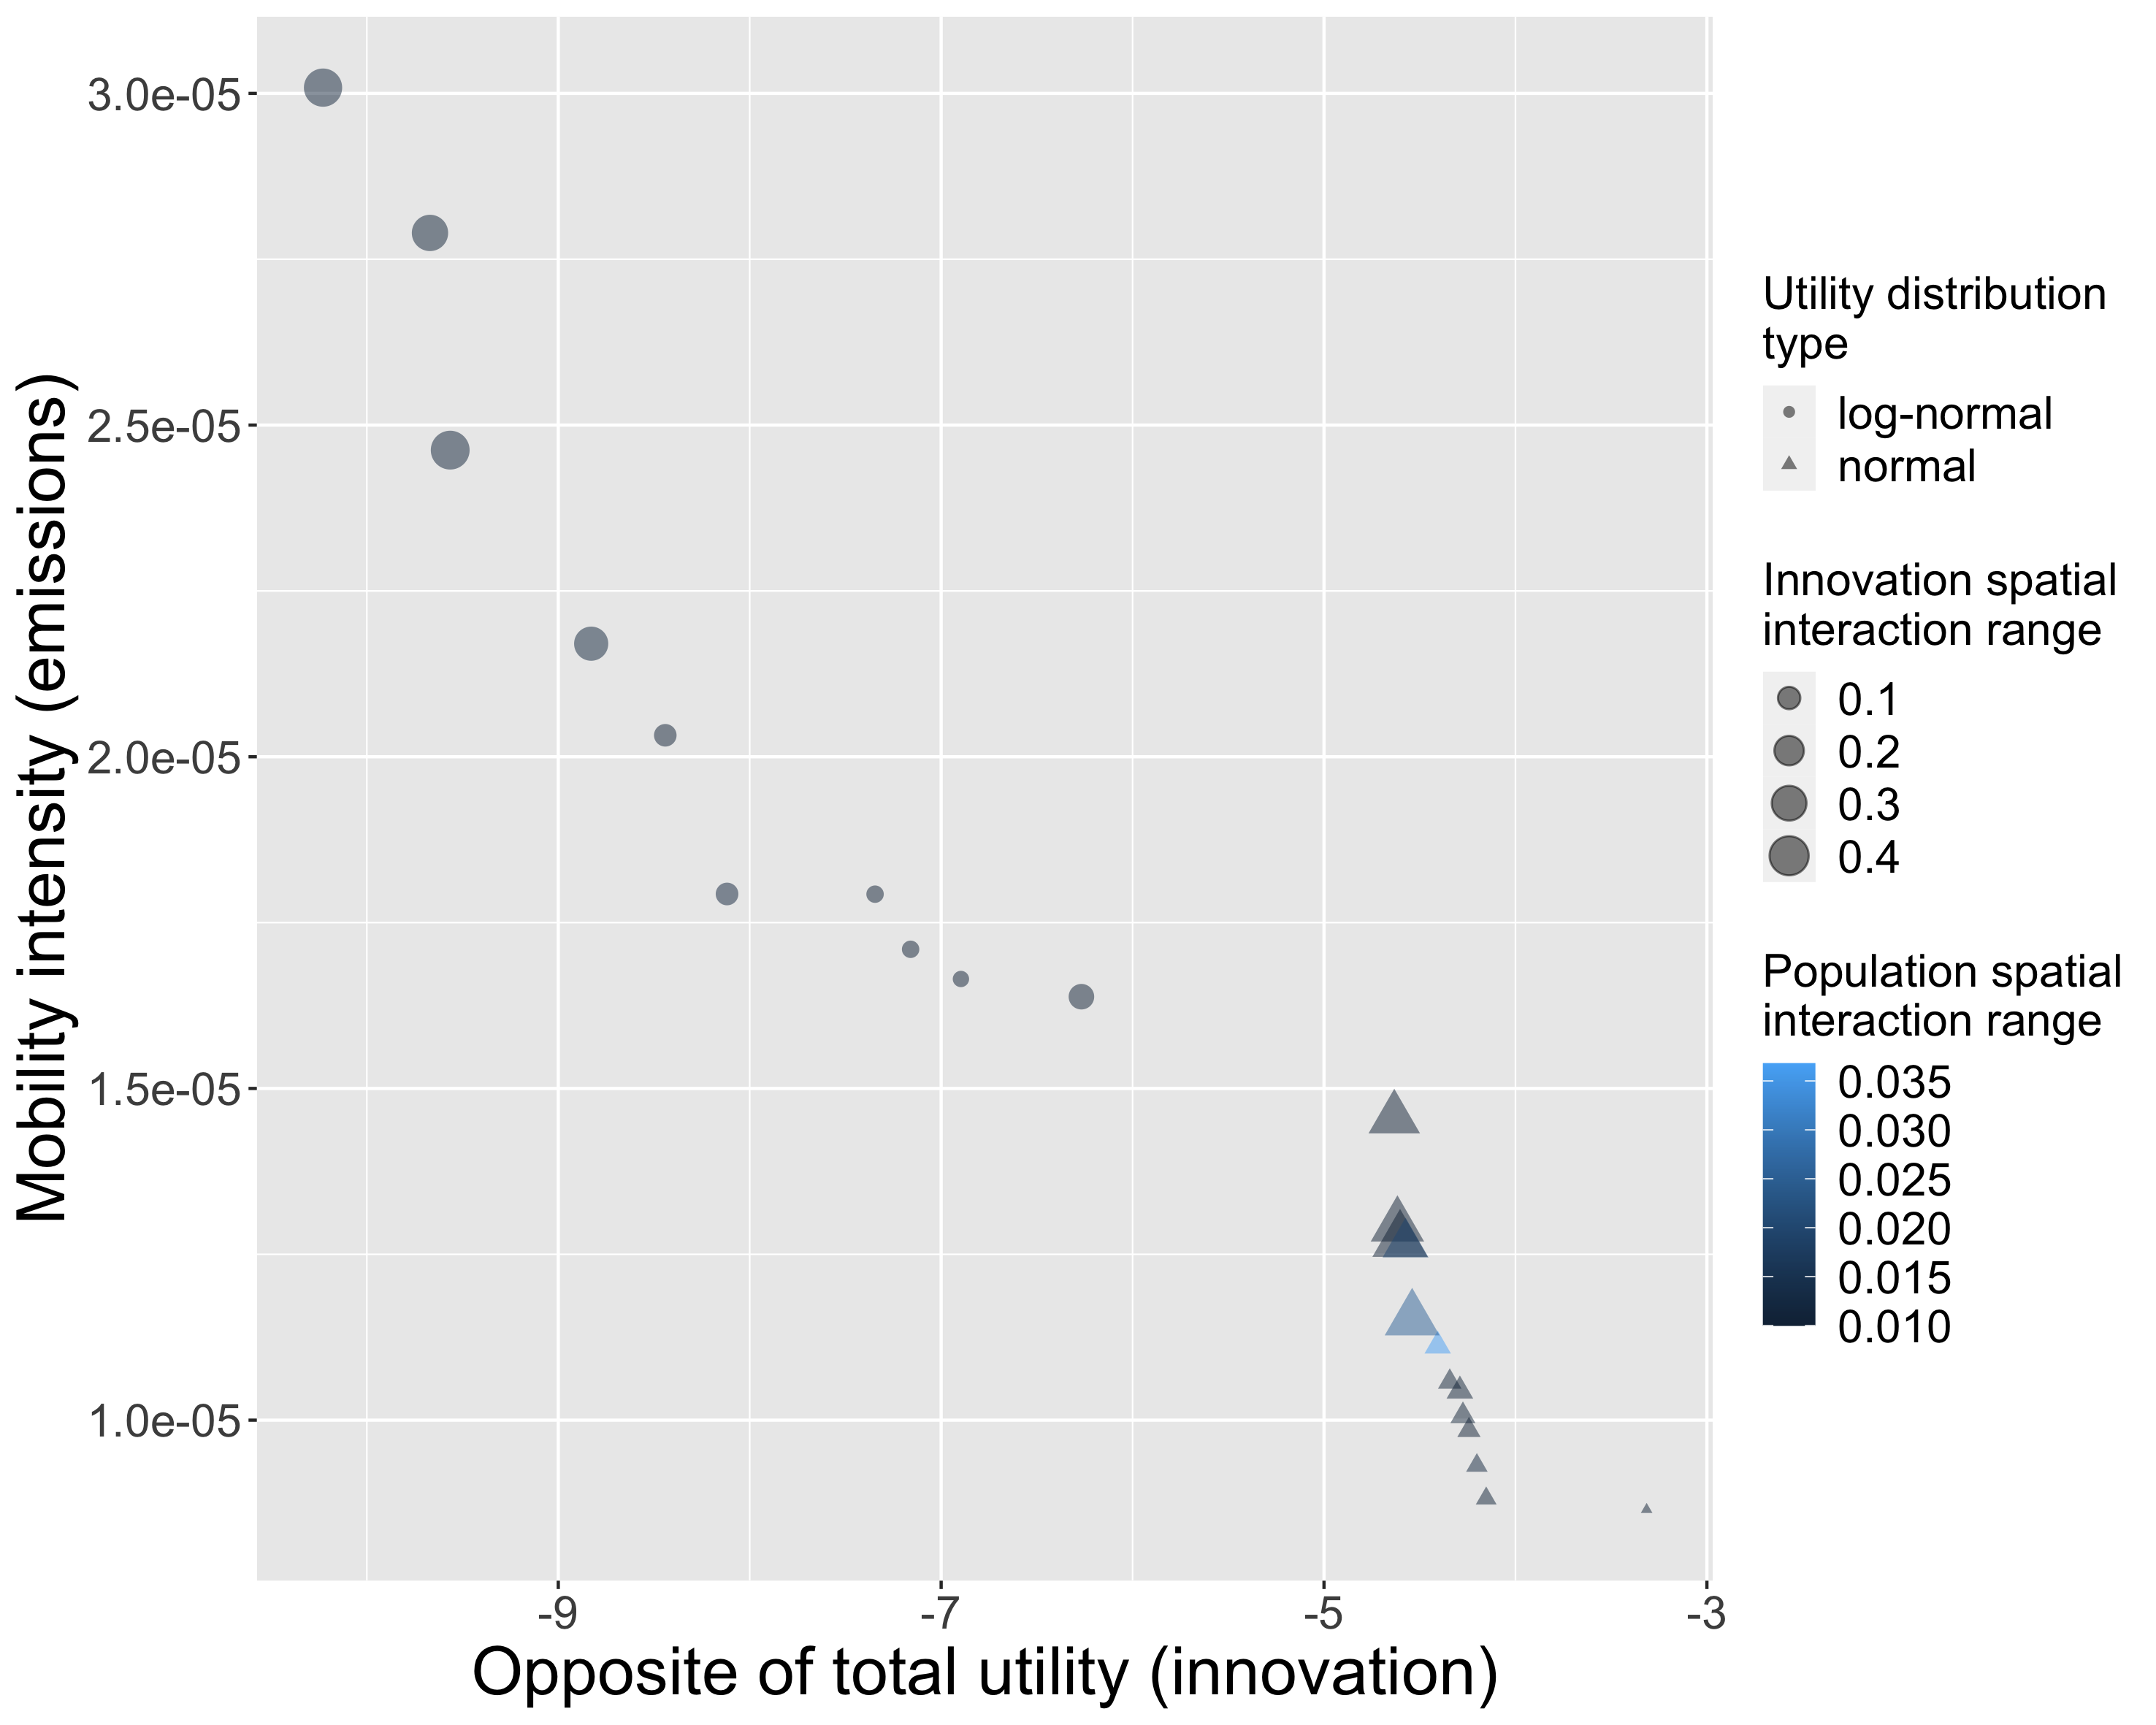
\includegraphics[height=0.7\textheight]{figures/pareto-oppAverageUtility-averageGravityFlow_color-gravityDecay_size-innovationDecay_shape-utilityDistribution.png}
\end{center}

\medskip

\textit{Pareto front confirms the existence of a trade-off}

% We indeed find a broad Pareto front, confirming the existence of a trade-off in such urban dynamics driven by innovation diffusion. We note two parts of the Pareto front, with fat-tailed distributions for utility distribution (log-normal) giving the upper part of the front corresponding to situations with a higher utility but which are more emission intensive. Within this subfront, population spatial interaction are rather local, while a more local innovation diffusion yields less emitting configurations. A similar aspect is observed for the normal distribution subfront, with a U-shaped value of population spatial interactions when going through the front: a more integrated system in terms of population migration produces by itself an intermediate compromise.

}

\sframe{Influence of urban hierarchy}{

\begin{center}
    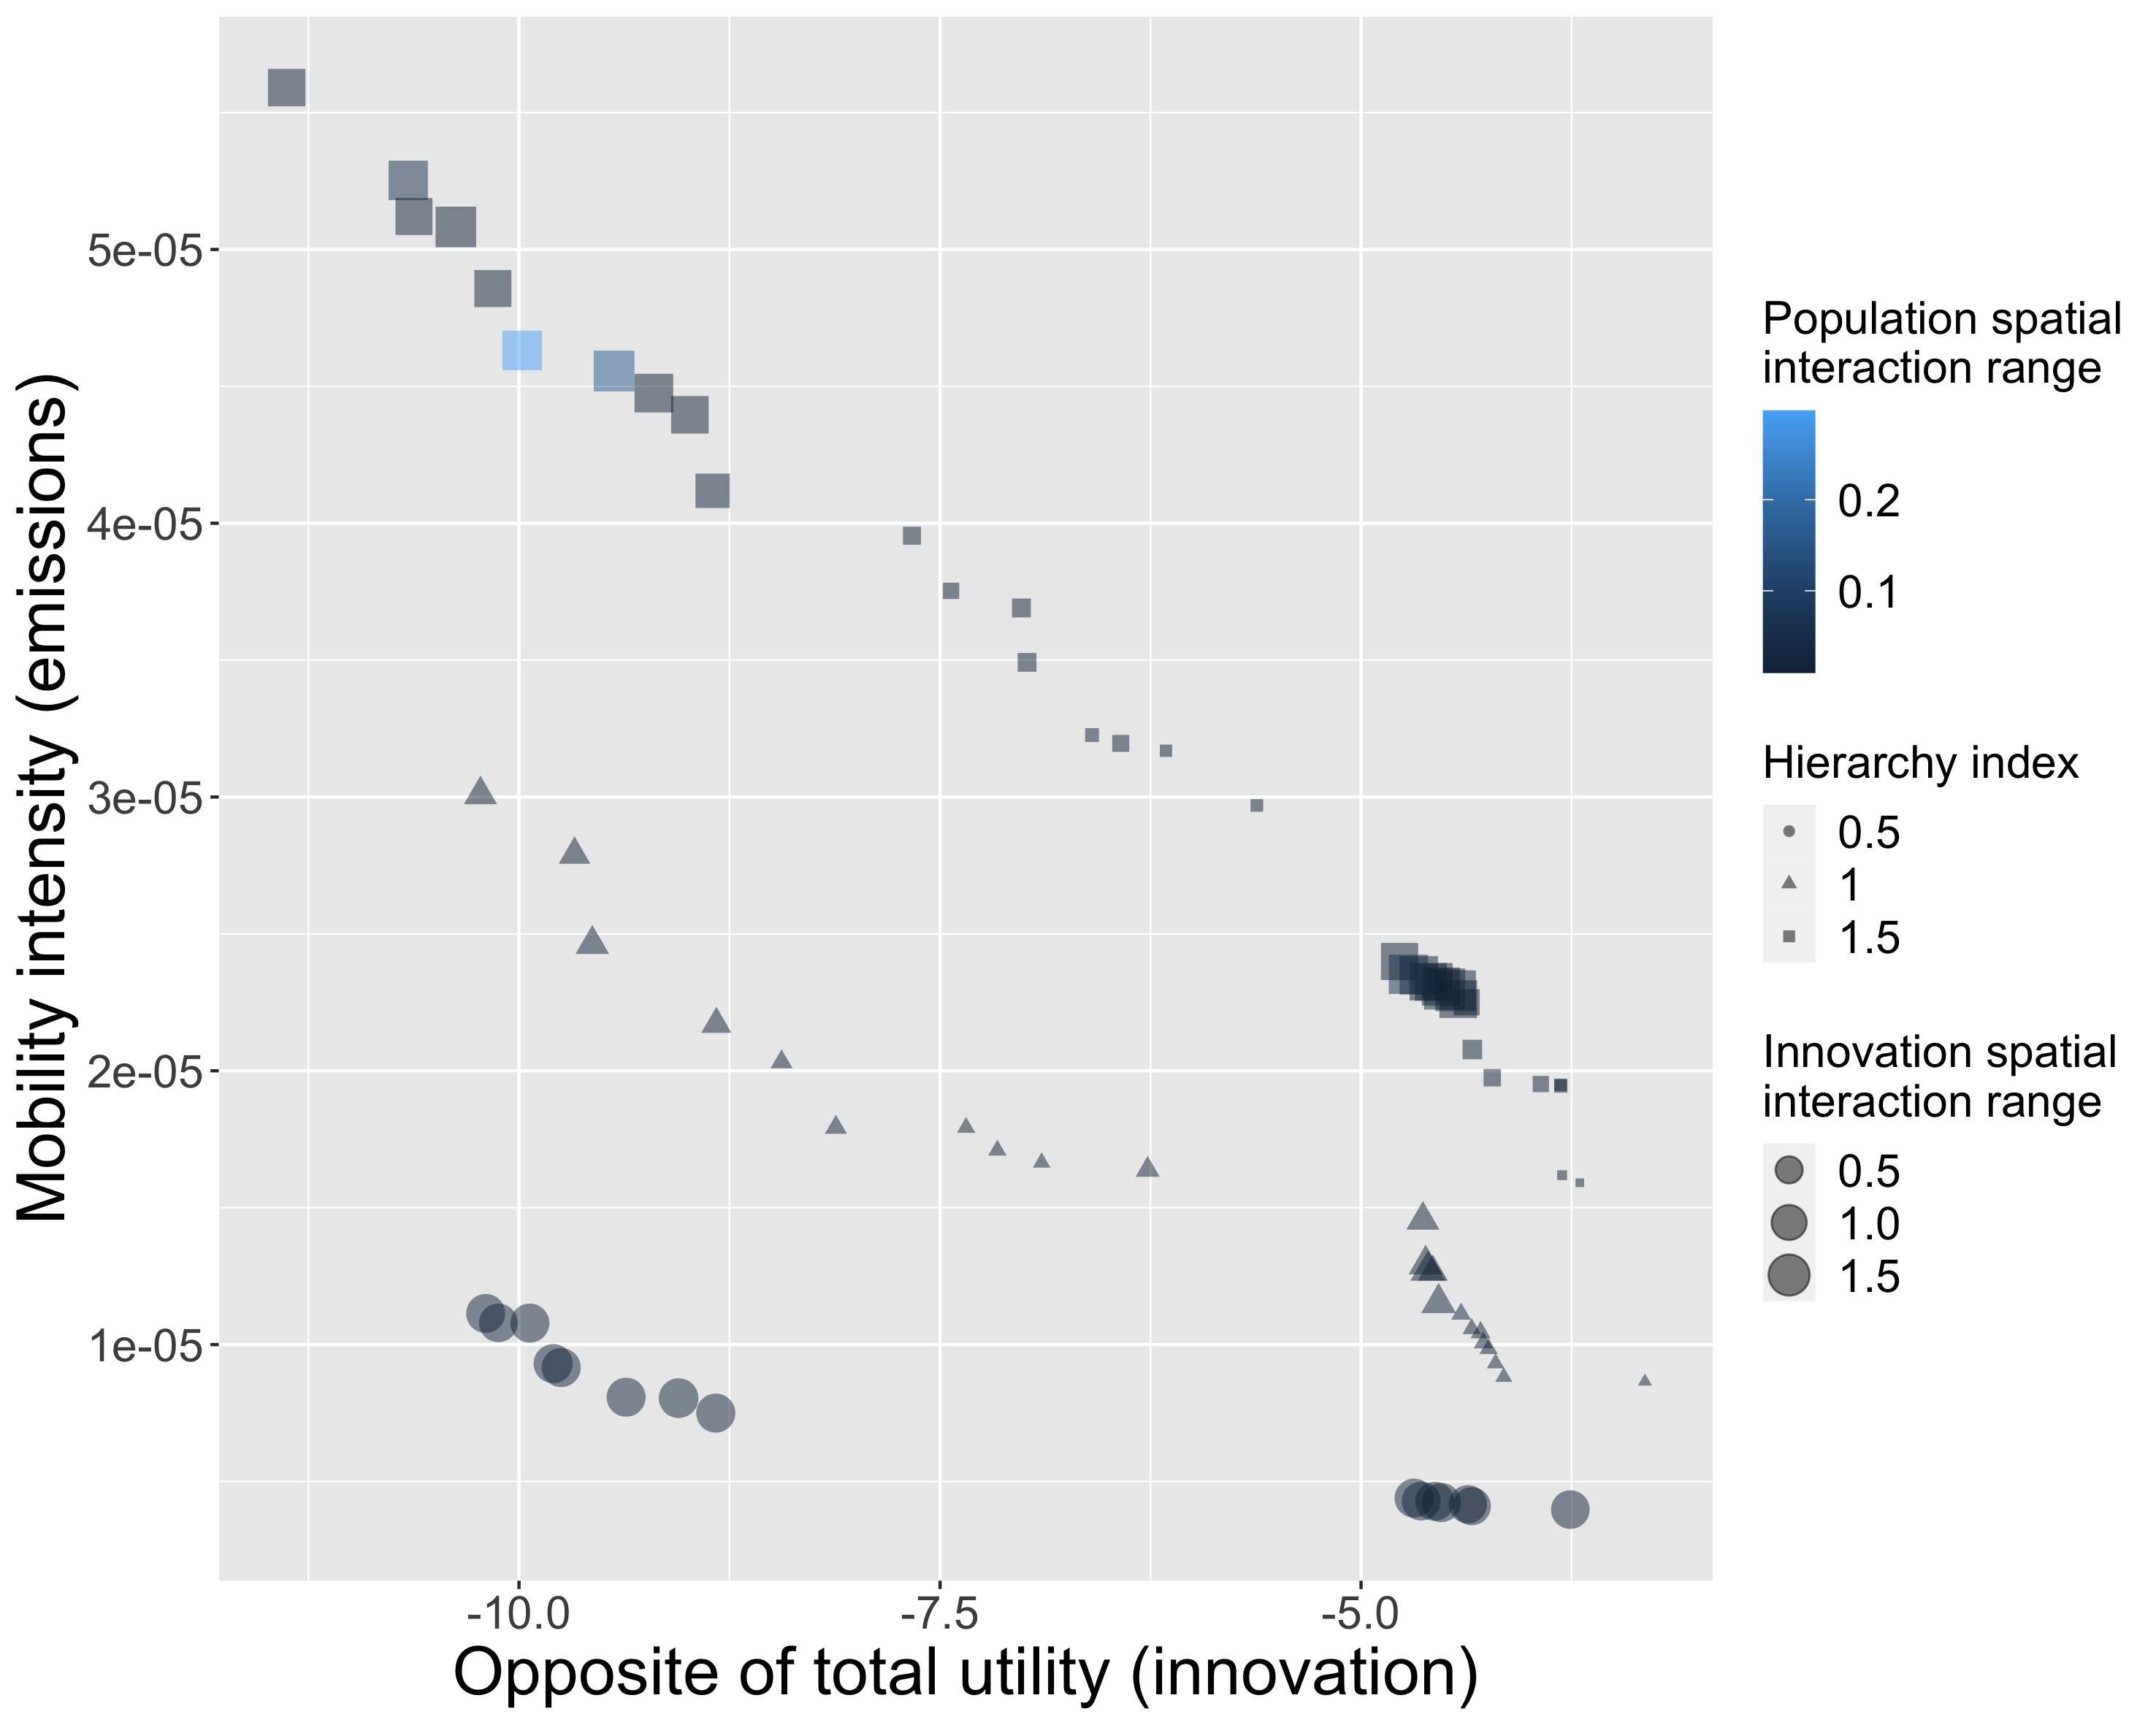
\includegraphics[height=0.7\textheight]{figures/pareto-oppAverageUtility-averageGravityFlow_VARYINGHIERARCHY_color-gravityDecay_size-innovationDecay.png}
\end{center}

\medskip

\textit{Higher inter-urban inequalities yield stronger trade-offs}

% We find that the higher the hierarchical inequalities, the less flat the front. Overall, the less hierarchical system dominates the others (but this comparison remains limited as total population is different across systems). Furthermore, the size of the front is the smallest with the less unequal hierarchy, meaning that this system is indeed closer to some global optimum.

}

\sframe{Influence of innovation hierarchy}{

\begin{center}
    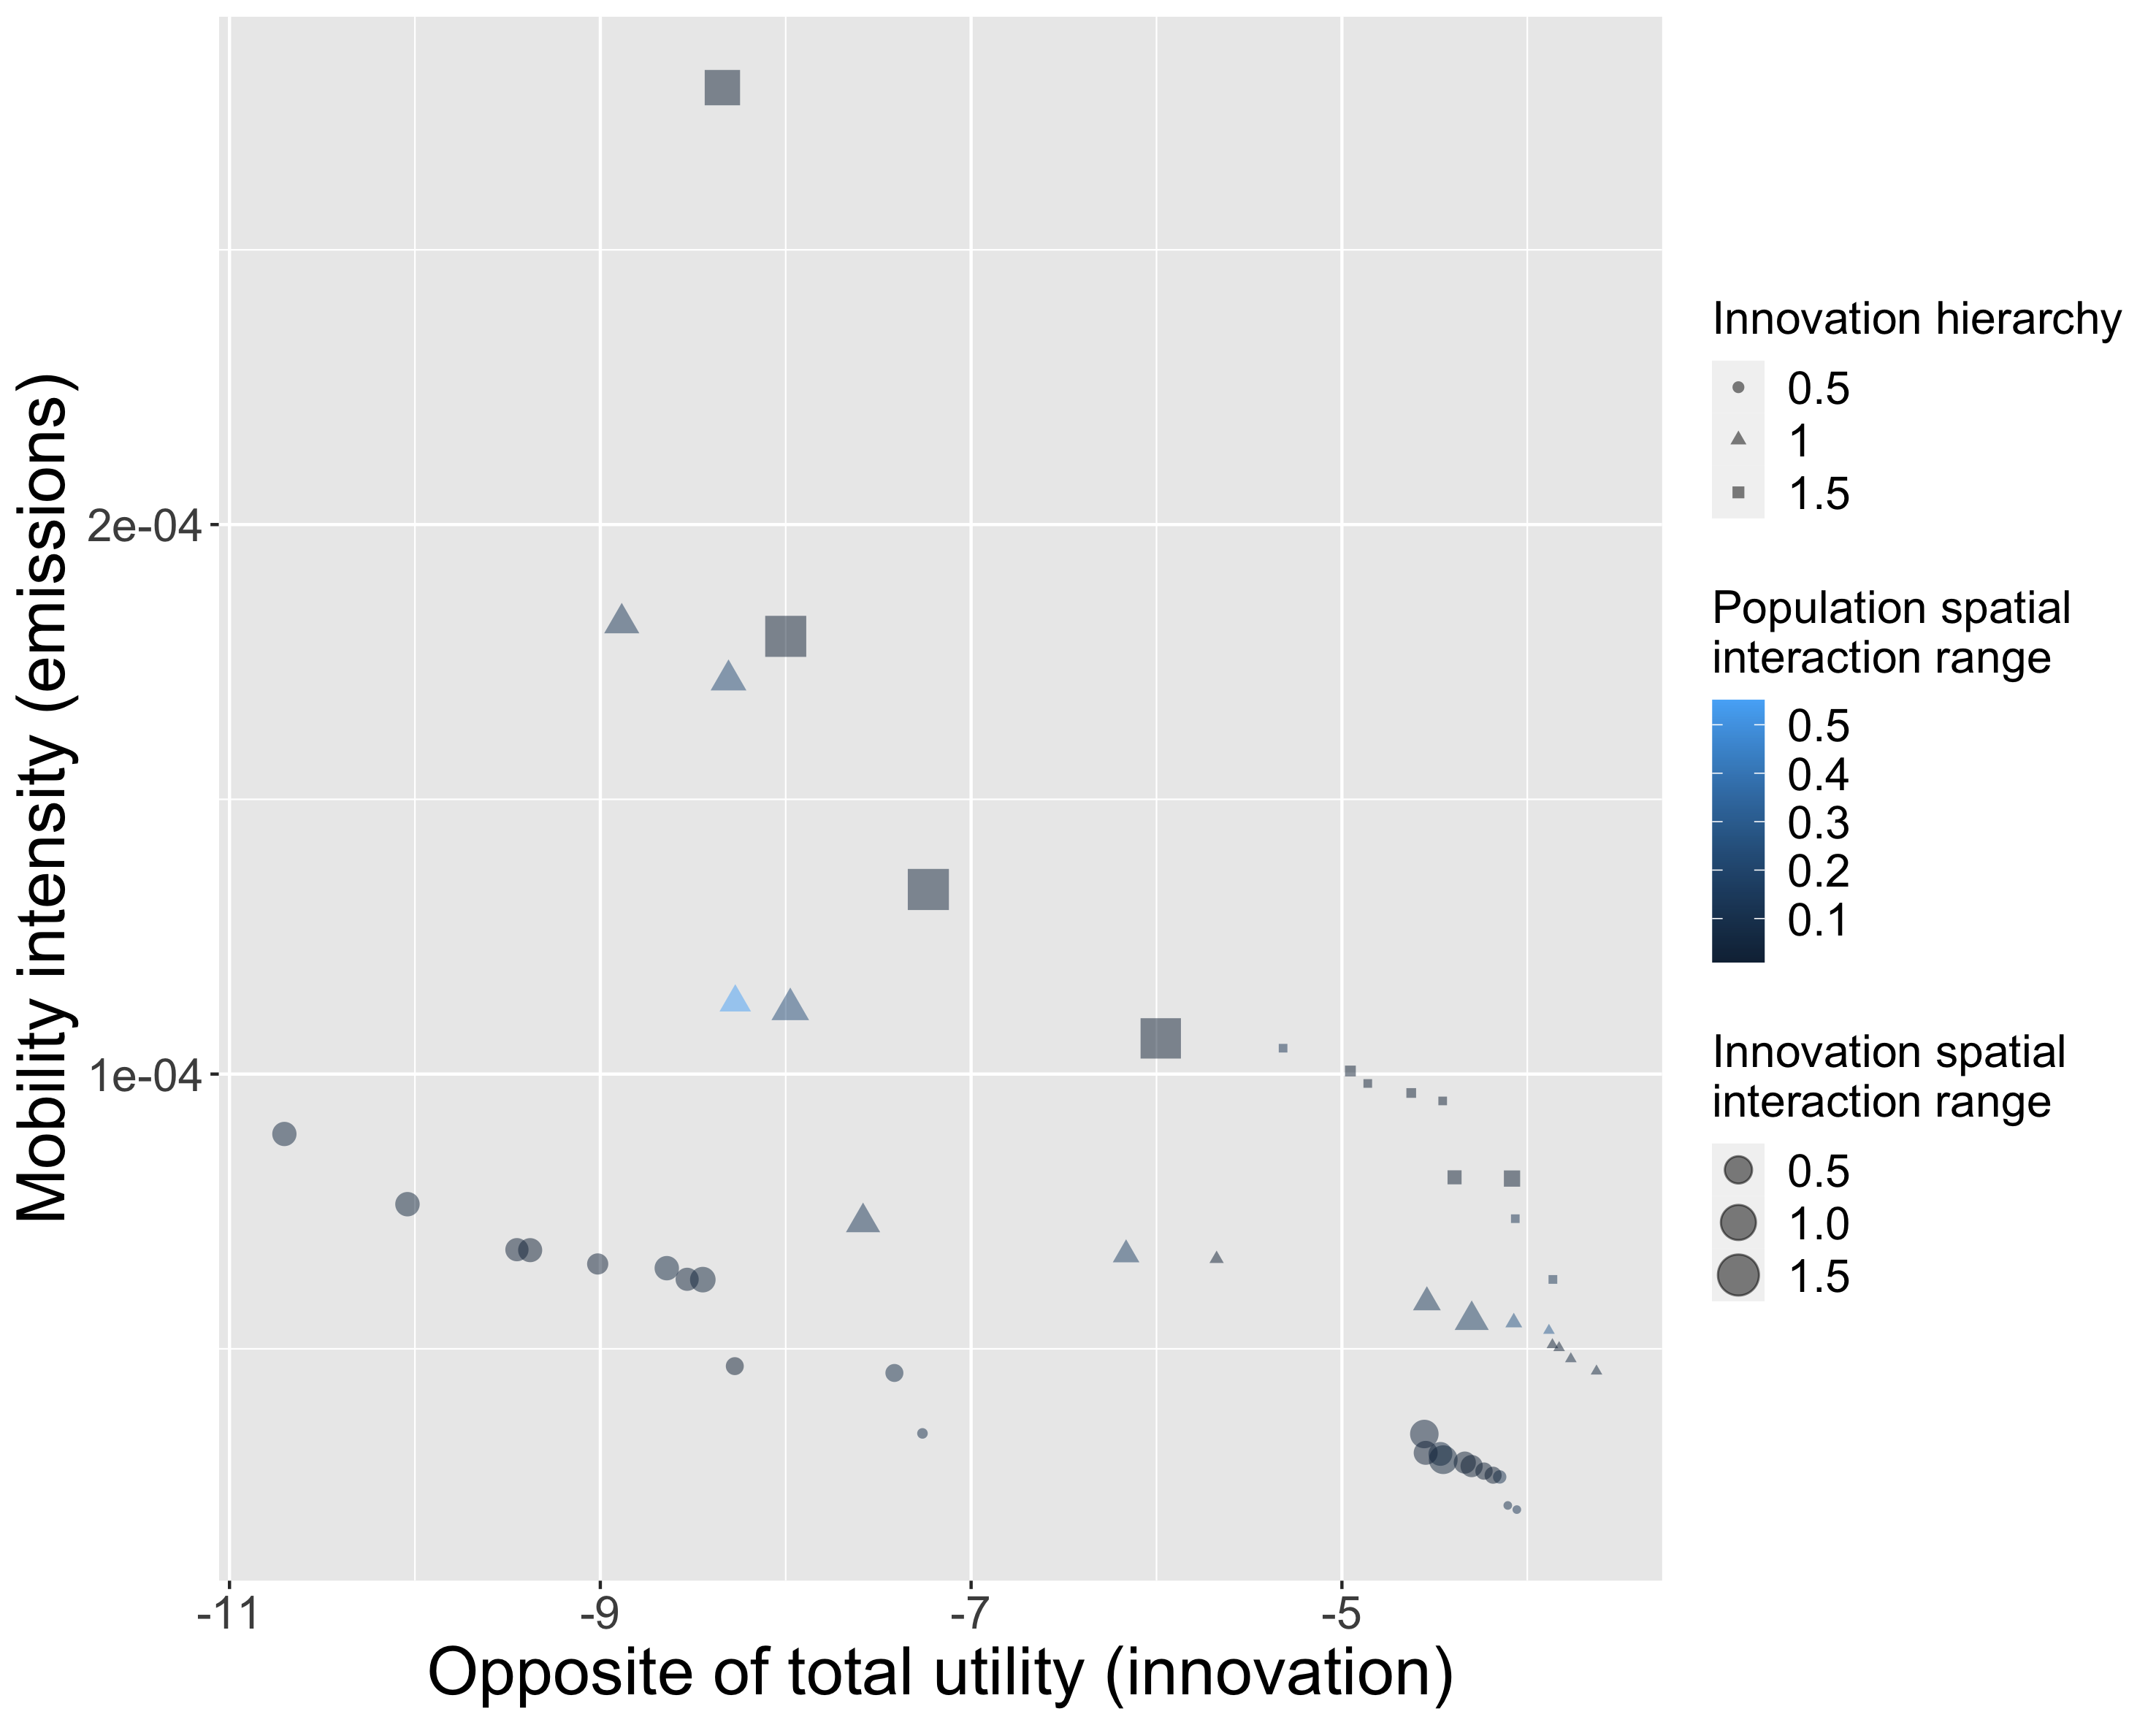
\includegraphics[height=0.7\textheight]{figures/pareto-oppAverageUtility-averageGravityFlow_VARYINGINNOVHIERARCHY_color-gravityDecay_size-innovationDecay.png}
\end{center}

\medskip

\textit{More balanced innovation yield higher utilities and less emissions (dominating Pareto front)}

%  We also find that balanced policies provides a more optimal front (they can be compared in this case). Furthermore, this lowest hierarchy corresponds to much higher absolute values of total utility, going against the narrative of a higher value innovation produced by large cities only. Points for the two other fronts are rather close, corresponding to a lower sensitivity when the scaling exponent is larger than one.

}






\sframe{Extension and link with empirical data}{

% Current work includes the extension of this model to additional dimensions of sustainable development goals such as accessibility and transport networks, economic prosperity and the reduction of inequalities, by coupling with other layers composed of analog models. We also explore the parametrisation and calibration of these models using real-world data, such as patents as a proxy for innovation and spatialised emissions. This works aims at paving the way towards multi-scale integrated models, applied to the design of sustainable territorial policies.

\textit{Work in progress:} empirical stylised facts on possible trade-offs in systems of cities; model parametrisation with real data (patents and spatialised emissions); extension to other SDGs.

\bigskip

\textbf{Issues:}

\medskip

\footnotesize

\begin{enumerate}
    \item Patent data as a proxy for innovation
    \begin{itemize}
        \item Geolocation of inventors not straightforward \cite{bergeaud2021patentcity,de2019geocoding}
        \item Which technological (sub-)classes? Model with one dimension (extension with a matrix genome?)
        \item Semantic content to better capture innovation diffusion? \cite{bergeaud2017classifying}
    \end{itemize}
    \item Emissions: inter-urban mobility emissions difficult to capture (need an additional transport model?)
    \item Additional dimensions: accessibility and public transport networks, economic prosperity and inequalities
    \begin{itemize}
        \item coupling with other layers for these dimensions \cite{raimbault2020empowering}
        \item many-objective optimisation? (NSGA3)
    \end{itemize}
\end{enumerate}

}







\section{Multiple models of city growth}



\sframe{City growth models: Gibrat's legacy}{


%\justify
\footnotesize

Simple law for city population growth proposed by R. Gibrat in 1931 \cite{gibrat1931inegalits} 

\[
\frac{P_i (t + 1) - P_i(t)}{P_i(t)} \sim \eta (t)
\]

\textit{Proportional growth: growth rates statistical distribution independent of city size}

%\cite{eeckhout2004gibrat} % comprehensive review - framing

\medskip

$\rightarrow$ Produces a log-normal size distribution \cite{eeckhout2004gibrat} (not a Pareto one - Zipf's law)

\medskip

$\rightarrow$ Extended model with minimal size for cities yields Zipf \cite{gabaix1999zipf}; other model with heterogenous variances \cite{cordoba2008generalized}

\medskip

$\rightarrow$ Empirical investigations confirm Gibrat's law seems to hold: US \cite{ioannides2003zipf}, France \cite{pumain1997city}, but not for China on some time periods \cite{ning2022urban}

\medskip

$\rightarrow$ Issues of city definition for estimation \cite{berry2012city} (as for scaling laws \cite{cottineau2017diverse})

}

\sframe{Simon and preferential attachment}{

Herbert Simon in 1955 proposed a model for city growth \cite{simon1955class}, which is analog to generalised preferential attachment with new entrants \cite{yamasaki2006preferential}

\bigskip
\bigskip

$\rightarrow$ Extended to include inter-city migrations \cite{haran1973modified}

\medskip

% equivalence of Gibrat and Simon

$\rightarrow$ Link between Gibrat model and generalised preferential attachment \cite{raimbault2018caracterisation}: preferential attachment at the individual level with strength $\lambda$ and new entrant probability $m$ yields a Gibrat's law in the limit $\lambda \ll 1$ such that

\[
\eta_i(t) = 1 + \frac{\lambda}{m \cdot (t - 1)}
\]


}

\sframe{Models benchmarking and validation issues}{

\footnotesize

% : towards multi-modeling?

\textbf{More elaborated extensions of city growth models, including urban interactions:}

\smallskip

% Pumain, Barth, Charlotte
Synergetics and migrations \cite{haag1992interurban}, urban dynamics based on spatial interactions \cite{pumain2012multi}, stochastic model with Taylor's law (conditional variance scales with average) \cite{james2018zipf}, stochastic model with migrations \cite{verbavatz2020growth}, \ldots


\bigskip

% how to benchmark models?
% - validation criteria: pop stat distrib only? dynamics? non-linear indics: rank?
% - which data to fit? just pop, or with mmigration? other dimmensions?
% - which systems of cities - def of cities - def of systemms - cf benchmark macro - geo case study
% - many exammple where models are commplementary - could be the same here? Then how to do umlti-modeling?

\textbf{How to benchmark and validate models?}

$\rightarrow$ Validation criteria: stationary distribution of population, dynamics, migrations, other dimensions (social, economic), non-linear indicators (rank dynamics), qualitative behavior, \ldots ?

\smallskip

$\rightarrow$ Data construction and quality: see Geodivercity ERC project \cite{pumain2020theories}

\smallskip

$\rightarrow$ Which geographical case studies: systems of cities, periods, definition of systems, of cities, \ldots ? \cite{raimbault2020empowering}

\smallskip

$\rightarrow$ Potential complementarity of models? Multi-modeling relevant at the mesoscopic scale for population density \cite{raimbault2020comparison}, road networks \cite{raimbault2021complementarity}, and building layouts \cite{raimbault2019generating}

}



\sframe{Conclusion}{

$\rightarrow$ \textbf{Integrated models} capturing complexity of \textbf{urban sustainability} towards \textbf{decision-making}.

\medskip

$\rightarrow$ \textbf{Robust} knowledge from models obtained with the development of \textbf{validation and exploration methods}.


\medskip

$\rightarrow$ \textbf{Complementarity} of perspectives, models and theories in an \textbf{interdisciplinary} context.

%\medskip

%$\rightarrow$ Which kind of interdisciplinarity?
% as a comment only: building bridges, while deep knowledge in each discipline? ~


\bigskip
\bigskip
\bigskip

\textbf{To use OpenMOLE (free and open software) and contribute: }\\
\url{https://next.openmole.org}

\bigskip

\textbf{Presented model open source at }

\url{https://github.com/JusteRaimbault/UrbanEvolution}

}









%%%%%%%%%%%%%%%%%%%%%
\begin{frame}[allowframebreaks]
\frametitle{References}
\bibliographystyle{apalike}
\bibliography{biblio}
\end{frame}
%%%%%%%%%%%%%%%%%%%%%%%%%%%%





\end{document}




